\documentclass[a4paper,11pt]{article}
\usepackage[a4paper,margin=2.4cm]{geometry}
\usepackage{amsmath,amssymb,amsthm}
\usepackage{fontspec}
\usepackage{unicode-math}
\usepackage{graphicx}
\usepackage{booktabs}
\usepackage{hyperref}
\usepackage{xcolor}
\definecolor{neonmagenta}{HTML}{FF10F0}
\usepackage{enumitem}
\usepackage{seqsplit}
\usepackage{fvextra}
% Allow long filenames to break across lines
\newcommand{\filename}[1]{\texttt{\seqsplit{#1}}}
% fvextra Verbatim for Lean listings (Unicode-safe, keeps characters in order)
\newcounter{leanlisting}
\newenvironment{leanlisting}[2]{%
  \refstepcounter{leanlisting}\label{#2}%
  \begin{center}\textit{\small Listing \theleanlisting: #1}\end{center}%
  \Verbatim[breaklines=true,breakanywhere=true,fontsize=\footnotesize,frame=single,framesep=4pt,rulecolor=\color{gray!50},fillcolor=\color{gray!5}]%
}{%
  \endVerbatim%
}
% Fonts (standing rule): Fira Sans (text), Fira Mono (code), Fira Math (math)
% only -- no other fonts for any reason. Math strokes very slightly
% emboldened (FakeBold=0.3); text untouched.
\setmainfont{Fira Sans}[BoldFont={Fira Sans Bold},ItalicFont={Fira Sans Italic},BoldItalicFont={Fira Sans Bold Italic}]
\setmonofont{Fira Mono}[BoldFont={Fira Mono Bold}]
\setmathfont{Fira Math}[FakeBold=0.3,Scale=1.15]
\hypersetup{colorlinks=true,linkcolor=blue!60!black,citecolor=blue!60!black,urlcolor=blue!60!black}
\setlength{\parskip}{0.6em}
\setlength{\parindent}{0pt}
\setlength{\emergencystretch}{2em}

\theoremstyle{plain}
\newtheorem{theorem}{Theorem}[section]
\newtheorem{proposition}[theorem]{Proposition}
\newtheorem{lemma}[theorem]{Lemma}
\newtheorem{corollary}[theorem]{Corollary}

\theoremstyle{definition}
\newtheorem{definition}[theorem]{Definition}

\theoremstyle{remark}
\newtheorem{remark}[theorem]{Remark}

\begin{document}

\title{\textbf{\Large Elimination of the GGHV Branch-(a,b) Normal Form at Degree~Pair $(72,108)$:}\\[0.6em]
\large A Certified Computational Audit\\[0.4em]
\normalsize Layer Reduction, Top-Layer Classification, and Final Obstruction}
\author{\textbf{Brandon D. McCrary}\\[0.25em]
\textit{Independent Researcher}\\[0.25em]
\href{https://orcid.org/0009-0008-2804-7165}{ORCID: 0009-0008-2804-7165}\\[0.6em]
{\small \parbox{0.92\textwidth}{\centering \textbf{Computation, Lean and LaTeX Source:}\\
{\color{neonmagenta}\hypersetup{urlcolor=neonmagenta}\href{https://github.com/brandonmccraryresearch-cloud/2D-Jacobian-Conjecture-Workspace}{\nolinkurl{https://github.com/brandonmccraryresearch-cloud/2D-Jacobian-Conjecture-Workspace}}}}}}
\date{September 28, 2026}
\maketitle

\begin{abstract}
We present a computational elimination of the branch~(a,b) normal form arising from Proposition~4.3 of Guccione--Guccione--Horruitiner--Valqui~\cite{GGHV} for a hypothetical $(72,108)$ counterexample to the planar Jacobian conjecture. Every base object is source-gated directly against GGHV v1 before any proof is drafted.

Starting from the verified Newton polygons
\[
\begin{aligned}
N(P)&=\operatorname{conv}\{(0,0),(1,0),(8,14),(8,16)\},\\
N(Q)&=\operatorname{conv}\{(0,0),(2,1),(12,21),(12,24)\},
\end{aligned}
\]
with $[P,Q]=x^2$ post-$\varphi$, we reduce the $72$-unknown bilinear system to five one-variable layers $E_1,\dots,E_5$ totaling $92$ equations, verified as an exact symbolic polynomial identity.

The top layer $E_5$ is the Davenport--Stothers extremal equation $\alpha\beta+u(2\alpha\beta'-3\alpha'\beta)=1$~\cite{Stothers,Davenport}. The Belyi classification gives the geometric upper bounds $3$, $10$, $35$ chart points for $m=3,5,7$; for $m=7$ the bound is sharp, with the degree-$35$ eliminating polynomial $\mathcal{W}(a_6)$ irreducible over $\mathbb{Q}$, a quintic in $S=a_6^7$ with nonzero discriminant and exactly one real root. The $35$ solutions are distinct and form a single Galois orbit: one real solution and $17$ conjugate pairs, grouped in five $S$-orbits. The classification is proved twice: the Belyi bound combined with the $35$ exhibited points gives a complete classification (relying on Riemann's existence theorem and the computed msolve parametrization), while \S\ref{sec:chartproof} gives an independent algebraic proof, valid over every field of characteristic~$0$, which is the route formalized in Lean. In reversed coordinates the chart equations are the coefficient recursion of $(1+y_1v+\dots+y_7v^7)^{3/2}$. Six weighted-homogeneous relations, of weights $4,5,5,6,6,7$ and with explicit certificates, cut out the five torus orbits. We formalize this proof in Lean.

The descent proceeds through $E_4$ (an $18\times19$ matrix of rank $17$, kernel dimension $2$), $E_3$ (a $19\times20$ matrix of rank $18$, kernel dimension $2$, unconditionally solvable for every direction $t$), and $E_2$ (injective $19\times 12$, rank $12$), leaving seven explicit compatibility conditions. We expand these as $b_i(t)+s_1M_i(t)+s_2L_i(t)=0$ with $b_i$ cubic and $M_i,L_i$ linear, eliminate $(s_1,s_2)$ to obtain $35$ quintic $3\times3$ minors. The entire descent is computed exactly over the quintic field $K_5$ in characteristic $0$: the $35$ minors span all binary quintics, forcing $t=0$. The case $t=0$ forces $B_0$ constant, contradicting the required vertex $(12,24)$. The Lean formalization quantifies over all roots of $R$ and all torus parameters, covering all $35$ top-layer solutions.

Hence no polynomials $P,Q$ satisfying $\mathrm{NewtonNF2}$ have $[P,Q]=\lambda x^2$ with $\lambda\neq0$ (Theorem~\ref{thm:main}). In Lean this NewtonNF2 form is a single kernel-checked theorem, \texttt{main\_theorem}, on the standard axioms only, independent of GGHV Proposition~4.3. Its top-layer input is \texttt{chartClassification\_holds}, a formalized algebraic proof of the $m=7$ top-layer classification of Proposition~\ref{prop:top-class}, in the normalized chart (\S\ref{sec:chartproof}). The further rigidity $a_{8,16}=0$ is an independent computer-algebra result (Corollary~\ref{cor:a816}). The application to the Jacobian conjecture is conditional on the correctness and exhaustiveness of~\cite[Proposition~4.3]{GGHV} (Corollary~\ref{cor:gghv}).
\end{abstract}

\vspace{1.2cm}
\hrule
\vspace{1.4cm}

\tableofcontents
\newpage

\section{Introduction}

\subsection{Context and prior work}

The planar Jacobian conjecture asserts that a polynomial map $(P,Q):\mathbb{C}^2\to\mathbb{C}^2$ with $[P,Q]:=P_xQ_y-P_yQ_x\in\mathbb{C}^\times$ is invertible. In~\cite{GGHV}, Guccione, Guccione, Horruitiner, and Valqui raise the lower bound on $\max\{\deg P,\deg Q\}$ for a hypothetical counterexample from $100$ (Moh~\cite{Moh}) to $108$, leaving open only the degree pair $(72,108)$ and its symmetric $(108,72)$.

Santib\'a\~nez-Leal has published machine evidence related to the $(72,108)$ candidate~\cite{Santibanez,SantibanezPaper}, explicitly not claiming elimination. The candidate itself is documented in~\cite{JC125note}.

For the degree pair $(72,108)$, \cite{GGHV} (an unrefereed preprint, arXiv:2204.14178v1) identifies two cases. The corner $(9,27)$ is discarded in \cite[\S5]{GGHV}; the open case is the corner $(8,28)$ with $(m,n)=(3,2)$. For this case, \cite[Proposition~4.3]{GGHV} shows that any counterexample gives rise, after an explicit (non-invertible) morphism $\varphi$, to one of two Newton polygon configurations. Case~(1), with additional vertices $(0,8)$ resp.\ $(0,12)$, is branch~(c). Case~(2), the subject of this paper, is branches~(a) and~(b):
\begin{equation}\label{eq:polygons}
\begin{aligned}
N(P)&=\operatorname{conv}\{(0,0),(1,0),(8,14),(8,16)\},\\
N(Q)&=\operatorname{conv}\{(0,0),(2,1),(12,21),(12,24)\},
\end{aligned}
\end{equation}
with $[P,Q]=x^2$ in post-$\varphi$ coordinates. See Figure~\ref{fig:polygons} for the polygon shapes.

\begin{figure}[htbp]
\centering
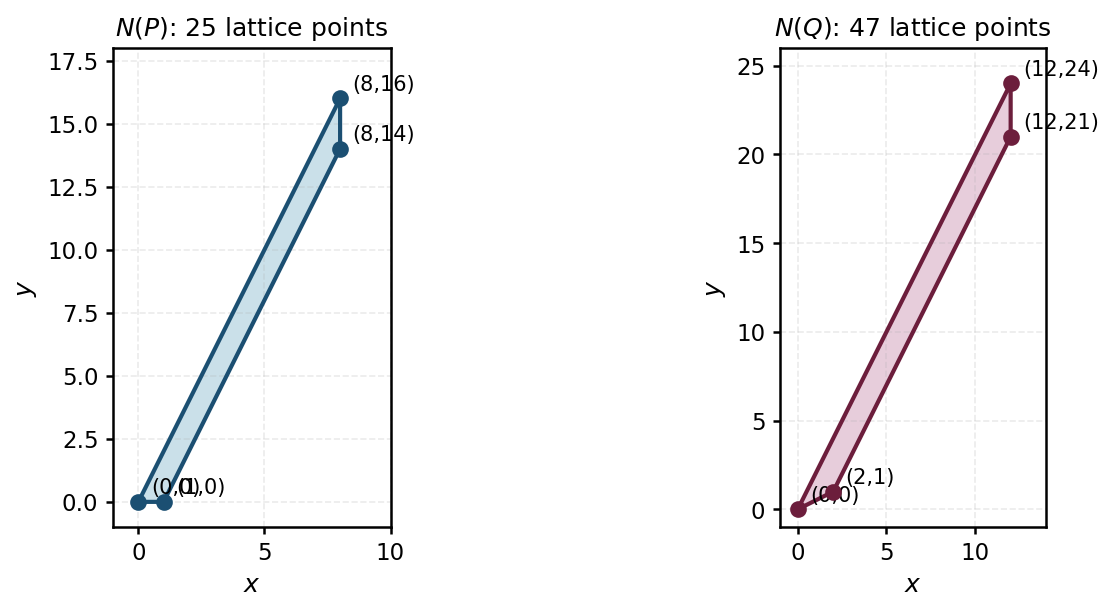
\includegraphics[width=0.95\linewidth]{figures/fig1_newton_polygons.png}
\caption{The branch~(a,b) Newton polygons from~\cite[Proposition~4.3(2)]{GGHV}, source-gated at v1 lines~495 and 599--600. $N(P)$ has $25$ lattice points; $N(Q)$ has $47$.}
\label{fig:polygons}
\end{figure}

\subsection{Main result}

\begin{theorem}[Elimination of the GGHV branch-(a,b) normal form]\label{thm:main}
Let $K$ be a field of characteristic~$0$. Let $P,Q\in K[x,y]$ have
$\operatorname{supp}P\subset N_P$ and $\operatorname{supp}Q\subset N_Q$,
with $a_{1,0}\cdot a_{8,14}\cdot b_{2,1}\cdot b_{12,21}\neq0$ and
$[P,Q]=\lambda x^2$ for some $\lambda\neq0$. Then $b_{12,24}=0$.
In particular, no $P,Q$ satisfy $\mathrm{NewtonNF2}(P,Q)$
(listing~\ref{lst:def-newtonnf2}; the polygons are in~\S\ref{sec:source})
with $[P,Q]=\lambda x^2$.
\end{theorem}

\begin{corollary}[Lower-edge rigidity]\label{cor:a816}
Under the hypotheses of Theorem~\ref{thm:main}, $a_{8,16}=0$ as well.
It rests on an explicit certificate over $K_5$ (\filename{scripts/a816\_certificate/}),
checked exactly by {\sc Singular} and by python-flint; it is not part of the Lean formalization;
see~\S\ref{sec:lower-edge}. It is not needed for the elimination: $b_{12,24}=0$
already contradicts the required Newton vertex $(12,24)$.
\end{corollary}

\begin{remark}[Lean-to-mathematics correspondence]\label{rem:nf2-bridge}
The Lean predicate \texttt{NewtonNF2} (listing~\ref{lst:def-newtonnf2}) is
\[
\texttt{NewtonNF2}(P,Q)\iff
\begin{cases}
\operatorname{supp}P\subseteq N_P,\ \operatorname{supp}Q\subseteq N_Q
\text{ (via \texttt{inNP}, \texttt{inNQ}),}\\
a_{0,0},a_{1,0},a_{8,14},a_{8,16}\neq0,\\
b_{0,0},b_{2,1},b_{12,21},b_{12,24}\neq0,
\end{cases}
\]
i.e.\ exactly the support conditions of Theorem~\ref{thm:main} together with the nonvanishing of the eight vertex coefficients. The half-plane predicates are tied to the vertex sets by \texttt{decide} checks run on duplicate predicates \texttt{latticeNP}/\texttt{latticeNQ} (which restate the same inequalities): the lattice-point counts ($25$ and $47$) and the vertex-membership check confirm the eight vertices lie on the polygons. This bridge is what lets the kernel-checked \texttt{main\_theorem} speak about the same $P,Q$ as Theorem~\ref{thm:main}.
\end{remark}

\begin{corollary}[Conditional on GGHV]\label{cor:gghv}
Assuming \cite[Prop.~4.3]{GGHV}, no counterexample to the plane Jacobian conjecture arises in case~$(8,28)$, sub-cases~a) and~b).
\end{corollary}

The proof is computational but exact. We reduce the $72$-unknown system to triangular layers (Figure~\ref{fig:layers}), determine the top layer via the Belyi-map/Riemann-existence argument (Figure~\ref{fig:top}), and independently by an algebraic argument formalized in Lean (\S\ref{sec:chartproof}). We then obstruct the descent via the Lean-formalized layer certificates (\S\ref{sec:descent}). Key steps were verified in {\sc Singular}~4.4.1 and Python/{\sc SymPy}; scripts are archived with this draft.

\begin{figure}[htbp]
\centering
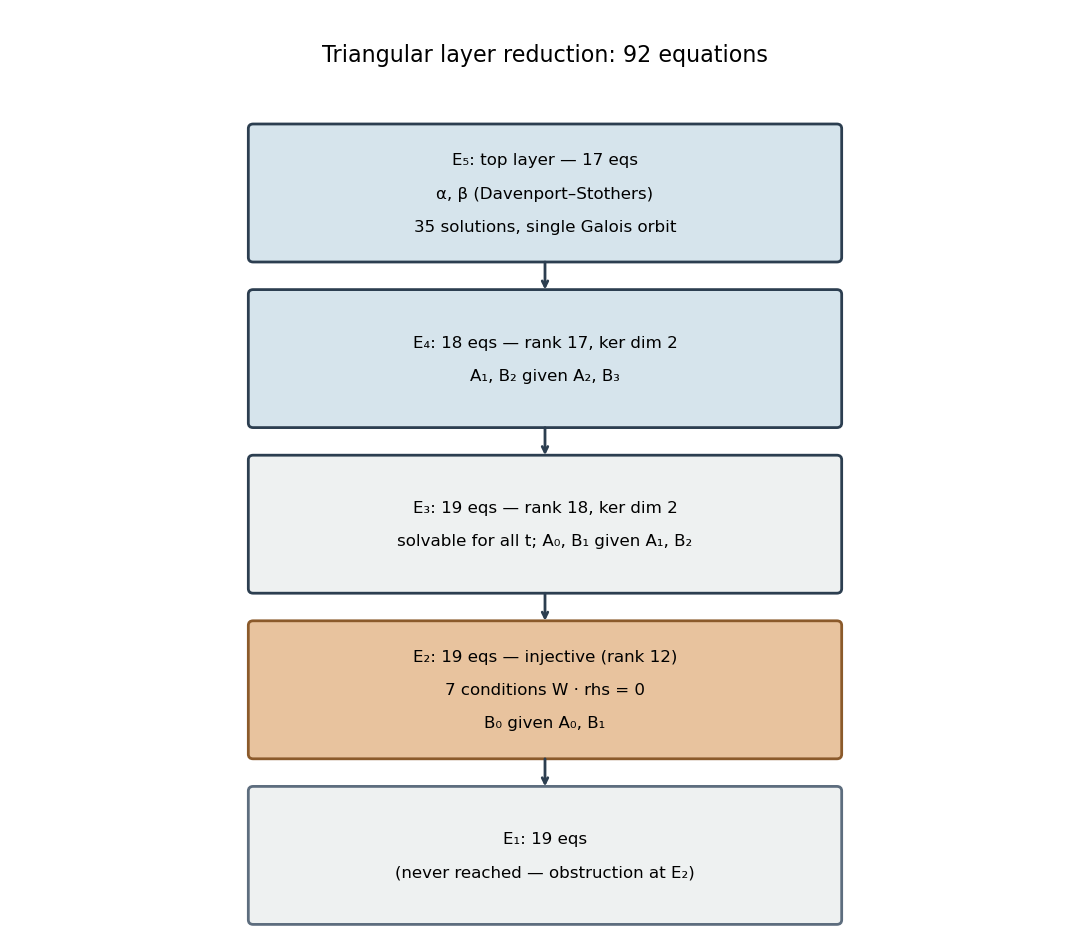
\includegraphics[width=0.75\linewidth]{figures/fig2_layer_descent.png}
\caption{The triangular layer structure: $92$ equations in five layers. Each layer is affine-linear in its unknowns given the solution above it.}
\label{fig:layers}
\end{figure}

\subsection{Logical status}

\begin{remark}\label{rem:conditional}
Theorem~\ref{thm:main} does not depend on GGHV. Its proof uses Proposition~6.1 for $m=7$,
which is proved twice. On paper it follows from Riemann's existence theorem
(\S\ref{sec:top}). In \S\ref{sec:chartproof} the classification it provides is proved
algebraically, in the normalized chart, and that proof is formalized in Lean as
\texttt{chartClassification\_holds} (listing~\ref{lst:proofchartclass}).
In Lean, \texttt{main\_theorem\_of\_chart} (listing~\ref{lst:chart}) derives the NewtonNF2 form of
Theorem~\ref{thm:main} from the explicit statement \texttt{ChartClassification}
(listing~\ref{lst:def-chartclass}). \texttt{main\_theorem} (listing~\ref{lst:unconditional})
combines it with \texttt{chartClassification\_holds} into a single kernel-checked
theorem independent of GGHV Proposition~4.3, and \texttt{\#print axioms} reports only \texttt{propext}, \texttt{Classical.choice}
and \texttt{Quot.sound}.
The $b_{12,24}=0$ part follows from \texttt{no\_completion\_K5\_PQ} together with \texttt{topLayerClassification\_of\_chart} and \texttt{chartClassification\_holds}; the $a_{8,16}=0$ part (Corollary~\ref{cor:a816}) rests on an explicit certificate $a_{8,16}^2=\sum_k H_k e_k$ over $K_5$, stored as the $76$ cofactors of $1=\sum_k z^2H_k e_k-(1+a_{8,16}z)(a_{8,16}z-1)$ in \filename{scripts/a816\_certificate/a816\_lift.txt} and checked exactly by {\sc Singular} and by python-flint; it is not formalized in Lean (see~\S\ref{sec:lower-edge}). Only Corollary~\ref{cor:gghv} also assumes GGHV
Proposition~4.3.
\end{remark}

\subsection{Outline}

Section~\ref{sec:source} source-gates all base objects against GGHV v1. Section~\ref{sec:system} sets up the $72$-unknown system. Section~\ref{sec:layers} gives the exact layer reduction. Section~\ref{sec:normalization} fixes normalizations. Section~\ref{sec:top} classifies the top layer. Section~\ref{sec:descent} carries out the descent. Section~\ref{sec:obstruction} proves the final obstruction. Section~\ref{sec:lifting} lifts to characteristic zero. Section~\ref{sec:conclusion} concludes and discusses the remaining branch~(c). Section~\ref{sec:attribution} covers prior work, attribution, and independence.

The proof is organized around four certificates. \emph{Certificate~I} (Newton reduction): $[P,Q]=\lambda x^2\Rightarrow E_5,\dots,E_1$ (\S\ref{sec:layers}). \emph{Certificate~II} (top-layer completeness): $E_5\Rightarrow$ five torus orbits over $K_5$ (\S\ref{sec:top}, \S\ref{sec:chartproof}). \emph{Certificate~III} (descent obstruction): $E_4,E_3,E_2\Rightarrow$ the compatibility ideal equals $(t_1,t_2)^5$, hence $t=0$ (\S\ref{sec:descent}, \S\ref{sec:obstruction}). \emph{Certificate~IV} (vertex destruction): $t=0\Rightarrow B_0'=0\Rightarrow b_{12,24}=0$ (Corollary~\ref{cor:t0}). The rigidity $a_{8,16}=0$ (Corollary~\ref{cor:a816}) is an independent supplementary result. The dependency graph is
\[
\boxed{\text{Counterexample in case }(8,28)\xrightarrow{\text{GGHV 4.3}} \text{NewtonNF2},\ [P,Q]=\lambda x^2 \xrightarrow{\text{Thm.~1.1}} \text{contradiction}}
\]
with Theorem~\ref{thm:main} itself independent of GGHV:
\begin{center}
\begin{tabular}{l|c}
\textbf{Result} & \textbf{Depends on GGHV?} \\ \midrule
Layer reduction & No \\
Top-layer classification & No \\
$K_5$ descent & No \\
$b_{12,24}=0$ & No \\
$a_{8,16}=0$ & No \\
Theorem~\ref{thm:main} & No \\
Corollary~\ref{cor:gghv} (Jacobian application) & Yes
\end{tabular}
\end{center}

\section{Source data}\label{sec:source}

We verify every base object directly against version~1 of~\cite{GGHV} (arXiv:2204.14178v1), downloaded from \url{https://arxiv.org/pdf/2204.14178v1} and extracted with \texttt{pdftotext -layout}. No proof is drafted until the polygons, bracket, and $\varphi$ are confirmed character-by-character against GGHV's text.

\begin{proposition}[{\cite[Proposition~4.3]{GGHV}, source-gated}]\label{prop:gghv43}
If there is a counterexample to the Jacobian conjecture in case~$(8,28)$, then there exist $P,Q\in L^{(1)}$ with $[P,Q]=x^2$ and one of:
\begin{itemize}[nosep]
\item[(1)] $N(P)=\{(0,0),(1,0),(8,14),(8,16),(0,8)\}$,\\
$N(Q)=\{(0,0),(2,1),(12,21),(12,24),(0,12)\}$;
\item[(2)] $N(P)=\{(0,0),(1,0),(8,14),(8,16)\}$,\\
$N(Q)=\{(0,0),(2,1),(12,21),(12,24)\}$.
\end{itemize}
\end{proposition}

\begin{proof}[Source locations]
The \texttt{pdftotext -layout} extraction of v1 yields:
\begin{itemize}[nosep]
\item Line~33: $[P,Q]:=P_xQ_y-P_yQ_x\in K^\times$ (bracket convention).
\item Line~492: ``Proposition~4.3 (Case $(8,28)$).''
\item Line~493: ``with $[P,Q]=x^2$'' (rendered as \texttt{x2} in the extraction).
\item Line~495: Case~(2) polygons\\
$N(P)=\{(0,0),(1,0),(8,14),(8,16)\}$, $N(Q)=\{(0,0),(2,1),(12,21),(12,24)\}$.
\item Lines~596--597: The morphism $\varphi(x)=x^{-1}$, $\varphi(y)=x^4y$; ``this is not an automorphism and the chain rule gives $[\varphi(P),\varphi(Q)]=-[P,Q]x^2$.''
\item Lines~599--600: ``in the cases a) and b) the Newton Polygons of $P$ and $Q$ become $N(P)=\{(0,0),(1,0),(8,14),(8,16)\}$, $N(Q)=\{(0,0),(2,1),(12,21),(12,24)\}$.''
\end{itemize}
A verification script (\filename{source\_gate\_verify.py}) asserts each of these lines automatically; it exits non-zero if any check fails.
\end{proof}

We work exclusively with case~(2) (branches~a,b).

\section{The polynomial system}\label{sec:system}

\subsection{Lattice points}

The Newton polygons~\eqref{eq:polygons} contain:
\begin{equation}
|N(P)\cap\mathbb{Z}^2|=25,\qquad |N(Q)\cap\mathbb{Z}^2|=47,
\end{equation}
verified by direct enumeration (cross-checked with Pick's theorem: $\operatorname{area}(N(P))=15$, boundary $18$, interior $7$). This gives $25+47=72$ unknown coefficients. The two constant terms do not appear in $[P,Q]$, leaving $70$ effective unknowns, but we retain all $72$ for the layer structure.

\subsection{The bracket equations}

Writing $P=\sum_{(i,j)\in N(P)}a_{ij}x^iy^j$ and $Q=\sum_{(i,j)\in N(Q)}b_{ij}x^iy^j$, the condition $[P,Q]=x^2$ expands to bilinear equations in the coefficients. Solving the full $72$-unknown bilinear system directly is impractical; we use the exact layer reduction of \S\ref{sec:layers}. (Direct expansion remains feasible for \emph{verification} of the reduction, as in Proposition~\ref{prop:layers}.)

\section{Exact layer reduction}\label{sec:layers}

Set $u=xy^2$ and decompose into $y$-layers:
\begin{equation}\label{eq:decomp}
P=\sum_{k} y^{-k}A_k(u),\qquad Q=\sum_{\ell} y^{-\ell}B_\ell(u),
\end{equation}
where $A_k,B_\ell\in\mathbb{C}[u]$ are one-variable polynomials whose coefficients are linear forms in the $a_{ij},b_{ij}$. The bracket $[P,Q]$ becomes a sum over $y$-layers, each a one-variable identity in $u$.

\begin{proposition}[Exact layer reduction]\label{prop:layers}
The system $[P,Q]=x^2$ on the $72$ coefficients implies five one-variable polynomial identities $E_1,\dots,E_5$ (the converse is not needed):
\begin{center}
\begin{tabular}{c|c|l}
\textbf{Layer} & \textbf{Equations} & \textbf{Unknowns (given previous layers)} \\
\midrule
$E_5$ & $17$ & Top: $\alpha,\beta$ \\
$E_4$ & $18$ & $A_1,B_2$ given $A_2,B_3$ \\
$E_3$ & $19$ & $A_0,B_1$ given $A_1,B_2$ \\
$E_2$ & $19$ & $B_0$ given $A_0,B_1$ \\
$E_1$ & $19$ & Lowest coefficients \\
\midrule
Total & $92$ & \\
\end{tabular}
\end{center}
The layer reduction was verified as a polynomial identity (script \filename{C1\_layer\_reduction.sing}) with all $72$ coefficients treated as symbolic indeterminates; the residual is identically zero.
\end{proposition}

\begin{proof}[Computational verification]
Substituting~\eqref{eq:decomp} into $[P,Q]-x^2$ and collecting by powers of $y$ yields the five identities $E_1,\dots,E_5$. Expanding each $E_i$ in the $72$ indeterminates and comparing coefficients with the direct bilinear expansion of $[P,Q]-x^2$ gives zero difference as a polynomial in $72$ variables. Script: \filename{C1\_layer\_reduction.sing} ({\sc Singular}).
\end{proof}

% BEGIN-MECHANICAL:lst:layers
\begin{leanlisting}{Mechanically extracted from \texttt{Jacobian/BranchAbLayers.lean} (sha256 \texttt{7c16141b4b126b3e}); statement verbatim, proof elided.}{lst:layers}
theorem layers_of_jac (lam : K) (A₀ A₁ A₂ B₀ B₁ B₂ B₃ : Polynomial K)
    (p₀ p₁ p₂ q₀ q₁ q₂ q₃ : MvPolynomial (Fin 2) K)
    (hp₀ : X 1 ^ 0 * p₀ = evH A₀) (hp₁ : X 1 ^ 1 * p₁ = evH A₁) (hp₂ : X 1 ^ 2 * p₂ = evH A₂)
    (hq₀ : X 1 ^ 0 * q₀ = evH B₀) (hq₁ : X 1 ^ 1 * q₁ = evH B₁) (hq₂ : X 1 ^ 2 * q₂ = evH B₂)
    (hq₃ : X 1 ^ 3 * q₃ = evH B₃)
    (hJ : jac (p₀ + p₁ + p₂) (q₀ + q₁ + q₂ + q₃) = C lam * X 0 ^ 2) :
    layerTerm 2 3 A₂ B₃ = Polynomial.C lam * Polynomial.X ^ 2 ∧
    layerTerm 2 2 A₂ B₂ + layerTerm 1 3 A₁ B₃ = 0 ∧
    layerTerm 2 1 A₂ B₁ + layerTerm 1 2 A₁ B₂ + layerTerm 0 3 A₀ B₃ = 0 ∧
    layerTerm 2 0 A₂ B₀ + layerTerm 1 1 A₁ B₁ + layerTerm 0 2 A₀ B₂ = 0 ∧
    layerTerm 1 0 A₁ B₀ + layerTerm 0 1 A₀ B₁ = 0 := by
  -- proof body elided (see artifact)
\end{leanlisting}
% END-MECHANICAL:lst:layers

The basic definitions used above are printed verbatim here, since only a human reader (not the Lean kernel) checks definitions:
% BEGIN-MECHANICAL:lst:def-jac
\begin{leanlisting}{Mechanically extracted from \texttt{Jacobian/BranchAbLayers.lean} (sha256 \texttt{7c16141b4b126b3e}); definition printed verbatim in full.}{lst:def-jac}
def jac (P Q : MvPolynomial (Fin 2) K) : MvPolynomial (Fin 2) K :=
  pderiv 0 P * pderiv 1 Q - pderiv 1 P * pderiv 0 Q
\end{leanlisting}
% END-MECHANICAL:lst:def-jac
% BEGIN-MECHANICAL:lst:def-uu
\begin{leanlisting}{Mechanically extracted from \texttt{Jacobian/BranchAbLayers.lean} (sha256 \texttt{7c16141b4b126b3e}); definition printed verbatim in full.}{lst:def-uu}
def uu : MvPolynomial (Fin 2) K := X 0 * X 1 ^ 2
\end{leanlisting}
% END-MECHANICAL:lst:def-uu
% BEGIN-MECHANICAL:lst:def-evh
\begin{leanlisting}{Mechanically extracted from \texttt{Jacobian/BranchAbLayers.lean} (sha256 \texttt{7c16141b4b126b3e}); definition printed verbatim in full.}{lst:def-evh}
def evH : Polynomial K →ₐ[K] MvPolynomial (Fin 2) K := Polynomial.aeval (uu (K := K))
\end{leanlisting}
% END-MECHANICAL:lst:def-evh
% BEGIN-MECHANICAL:lst:def-layerterm
\begin{leanlisting}{Mechanically extracted from \texttt{Jacobian/BranchAbLayers.lean} (sha256 \texttt{7c16141b4b126b3e}); definition printed verbatim in full.}{lst:def-layerterm}
def layerTerm (a b : ℕ) (A B : Polynomial K) : Polynomial K :=
  (a : Polynomial K) * A * Polynomial.derivative B - (b : Polynomial K) * Polynomial.derivative A * B
\end{leanlisting}
% END-MECHANICAL:lst:def-layerterm

The system is triangular (Figure~\ref{fig:layers}): $E_5$ involves only the top-layer unknowns, and each $E_i$ ($i<5$) is affine-linear in its unknowns given a solution of the layers above. This is the key structural fact that makes the problem tractable. Conceptually, the Newton polygons induce a weighted grading, and the Jacobian equation respects that grading: the five $E_i$ are the homogeneous components of $[P,Q]=x^2$ with respect to it. The triangular structure is thus not a computational accident but a structural consequence of the grading, and the operator $\mathrm{LT}_{a,b}(A,B)=aAB'-bA'B$ is its homogeneous bracket.

\section{Normalization}\label{sec:normalization}

The top-layer unknowns admit rescaling symmetries from the torus action. We fix, without loss of generality,
\begin{equation}\label{eq:normalization}
a_{1,0}=a_{8,14}=1,
\end{equation}
leaving $a_{8,16}$ free. The remaining $1$-dimensional torus acts by the $Y$-weight grading used in the layer decomposition (\S\ref{sec:layers}); the finite subgroup $\mu_7$ gives $7$ chart copies per orbit.

\begin{remark}[Lean chart normalization]
The Lean formalization uses chart coordinates $(a_1,\dots,a_7,b_0,\dots,b_9)$ with the torus normalization $a_7^3 b_0^2 = 1$ (see \texttt{ChartClassification} in \texttt{Jacobian/BranchAbChart.lean}). After fixing $\alpha_0 = 1$ and $\beta_{10} = 1$, the remaining scaling $u \mapsto \kappa u$ acts on $a_7$ with weight~$7$ and on $b_0$ with weight~$-10$, hence on $a_7^3 b_0^2$ with weight $21 - 20 = 1$. The condition $a_7^3 b_0^2 = 1$ therefore fixes $\kappa$ completely, with no $7$th-root ambiguity: the Lean chart meets each torus orbit \emph{exactly once}, giving $5$ points, not $35$. The \S\ref{sec:normalization} chart ($a_{1,0} = a_{8,14} = 1$) meets each orbit $7$ times. The two charts are related by a torus element requiring a $7$th root.
\end{remark}

\emph{Vertex conditions used.}\label{sec:lower-edge} The proof uses $(1,0)$ and $(2,1)$ (equivalently $\lambda\neq0$), $(8,14)$ (normalization and top-layer degree), and $(12,24)$ (the $t=0$ exclusion). The vertex $(8,16)$ is left free in the Lean formalization; however, an explicit certificate over $K_5$ (Corollary~\ref{cor:a816}; \filename{scripts/a816\_certificate/}, checked exactly by {\sc Singular} and by python-flint) shows that $a_{8,16} = 0$ is forced once $E_1$ is included, giving a second independent contradiction from the lower edge.

% BEGIN-MECHANICAL:lst:torus
\begin{leanlisting}{Mechanically extracted from \texttt{Jacobian/BranchAbTorus.lean} (sha256 \texttt{97918673d5c4dc09}); statement verbatim, proof elided.}{lst:torus}
theorem layers_transport (α β κ : K) (A₀ A₁ A₂ B₀ B₁ B₂ B₃ : K[X])
    (E4 : layerTerm 2 2 A₂ B₂ + layerTerm 1 3 A₁ B₃ = 0)
    (E3 : layerTerm 2 1 A₂ B₁ + layerTerm 1 2 A₁ B₂ + layerTerm 0 3 A₀ B₃ = 0)
    (E2 : layerTerm 2 0 A₂ B₀ + layerTerm 1 1 A₁ B₁ + layerTerm 0 2 A₀ B₂ = 0) :
    layerTerm 2 2 (C α * sc κ A₂) (C β * sc κ B₂) + layerTerm 1 3 (C α * sc κ A₁) (C β * sc κ B₃) = 0 ∧
    layerTerm 2 1 (C α * sc κ A₂) (C β * sc κ B₁) + layerTerm 1 2 (C α * sc κ A₁) (C β * sc κ B₂) +
      layerTerm 0 3 (C α * sc κ A₀) (C β * sc κ B₃) = 0 ∧
    layerTerm 2 0 (C α * sc κ A₂) (C β * sc κ B₀) + layerTerm 1 1 (C α * sc κ A₁) (C β * sc κ B₁) +
      layerTerm 0 2 (C α * sc κ A₀) (C β * sc κ B₂) = 0 := by
  -- proof body elided (see artifact)
\end{leanlisting}
% END-MECHANICAL:lst:torus

\section{The top layer}\label{sec:top}

\subsection{The Davenport--Stothers equation}

The top identity $E_5$ takes the form
\begin{equation}\label{eq:e5}
\alpha\beta+u\,(2\alpha\beta'-3\alpha'\beta)=1,
\end{equation}
where $\alpha=A_2/u$ and $\beta=B_3/u^2$ are polynomials of degree $7$ and $10$ respectively, the degrees being forced by the vertices $(8,14)\in N(P)$ and $(12,21)\in N(Q)$.

Setting $u=s^2$ with $f(s)=\alpha(s^2)$ and $g(s)=s\beta(s^2)$, equation~\eqref{eq:e5} becomes the Davenport--Stothers extremal equation~\cite{Stothers,Davenport}
\begin{equation}
2fg'-3f'g=c\neq0.
\end{equation}
Indeed $2fg'-3f'g=2(\alpha\beta+u(2\alpha\beta'-3\alpha'\beta))$. With $\deg f=14=2k$ and $\deg g=21=3k$ ($k=7$), we have $\deg(g^2-c\cdot f^3)=8=k+1$, which is exactly Davenport's bound: the pair is extremal.
with $f$ even and $g$ odd. Here $\deg_s f = 2m$ where $m=\deg_u\alpha$; the relation $1+2n-3m=0$ (with $n=\deg_u\beta$) forces $m$ odd. The cases $m=1,3,5,7$ admit solutions; $m=7$ is the relevant case for~\eqref{eq:polygons}. The symmetric (parity-constrained) classification is computed here via elimination; we do not claim it follows from the literature.

\subsection{Classification}

\begin{proposition}[Top-layer solutions]\label{prop:top-class}
The system $E_5$ has:
\begin{itemize}[nosep]
\item $m=3$: $3$ complex solutions; eliminant $3a_2^3-32$, irreducible over $\mathbb{Q}$;
\item $m=5$: $10$ complex solutions; eliminant $9a_4^{10}+37200a_4^5+95051008$, irreducible over $\mathbb{Q}$;
\item $m=7$: $35$ complex solutions; eliminant $\mathcal{W}(a_6)$ of degree $35$.
\end{itemize}
The $m=7$ case is the one relevant to~\eqref{eq:polygons}.
\end{proposition}

\begin{proof}
We work over~$\mathbb{C}$: the Belyi classification is topological, hence valid over~$\mathbb{C}$, and the resulting count of solutions transfers to any field of characteristic~$0$ by base change (the equations are defined over~$\mathbb{Q}$). We normalize the third branch point to $c=1$ by the scaling $u\mapsto c\,u$, which preserves the torus action. We prove the counts in characteristic~$0$ via the Belyi-map classification. For the top layer, $E_5$ is $\alpha\beta+u(2\alpha\beta'-3\alpha'\beta)=1$ with $\deg\alpha=m$, $\deg\beta=(3m-1)/2$ ($m=3,5,7$, so $\deg\beta=4,7,10$). Put $\varphi=u\beta^2/\alpha^3$. Then $\varphi'=\beta E/\alpha^4=\beta/\alpha^4$, so $\varphi$ is a Belyi map: it ramifies only over $0$, $\infty$, and $c=\varphi(\infty)\neq0$. The ramification is forced as follows. At a root $r$ of $\alpha$, $E(r)=-3r\cdot\alpha'(r)\beta(r)=1$. So $\alpha$ has simple nonzero roots, none shared with $\beta$. At a root $s$ of $\beta$, $E(s)=2s\cdot\alpha(s)\beta'(s)=1$, so $\beta$ also has simple nonzero roots. Hence $\deg\varphi=3m$, and $\varphi'=\beta/\alpha^4$ vanishes in $\mathbb{C}$ only at the roots of $\beta$, which forces the passport
\[
\begin{array}{c|ccc}
m=3 & [2^4 1]\;(n=9) & [3^3] & [7\cdot 1^2]\\
m=5 & [2^7 1]\;(n=15) & [3^5] & [12\cdot 1^3]\\
m=7 & [2^{10}1]\;(n=21) & [3^7] & [17\cdot 1^4]
\end{array}
\]
By Riemann's existence theorem, covers with this passport correspond to $S_n$-conjugacy classes of transitive triples in $C_0\times C_1\times C_\infty$ with product~$1$ (here $n=3m$). The Frobenius character formula (computed exactly in \filename{belyi\_counts\_m357.py} via the Murnaghan--Nakayama rule) counts $N$ triples with $N=9!$, $2\cdot15!$, $5\cdot21!$ for $m=3,5,7$; since every such triple has trivial centralizer, each $S_n$-conjugacy class has $n!$ elements, giving $N/n!=1$, $2$, $5$ covers. Every triple counted is transitive, for general~$m$: a non-transitive triple would have an orbit on which $g_\infty$ acts trivially, so on that orbit $g_0=g_1^{-1}$; but $g_1$ has cycle type $3^m$ (hence fixes no point, and so does $g_1^{-1}$), while $g_0$ has cycle type $2^{(3m-1)/2}1$ and contains no $3$-cycle---a contradiction. Hence all counted triples are genuine covers. Each cover has trivial automorphism group: an automorphism $u\mapsto\kappa u$ acts freely on the $m$ poles and on the $(m+1)/2$ unramified points over $c$, so its order divides $\gcd(m,(m+1)/2)=1$.

Now suppose two solutions give isomorphic covers. The isomorphism fixes the unique unramified point over $0$ ($u=0$) and the unique maximally ramified point over $c$ ($u=\infty$). So it is $u\mapsto\kappa u$, and comparing zeros and poles shows the two solutions differ by the torus action. Hence distinct orbits give non-isomorphic covers, and there are at most $m\cdot(\#\text{covers})$ chart points: $3$, $10$, $35$.

For $m=7$, the exactly verified parametrization (script \filename{verify\_msolve\_param.py}, shipped with inputs \filename{e5\_m7.ms} and \filename{e5\_m7.out} in \filename{scripts/}) exhibits $35$ distinct points, so the classification is complete in characteristic~$0$. For $m=3$ and $m=5$ the Belyi bound is likewise sharp. In the normalization $\alpha_0=\beta_0=\alpha_m=1$ the system is zero-dimensional, of vector-space dimension~$3$ for $m=3$ and $10$ for $m=5$; hence the solution set is nonempty and has at most $d$ points, where $d=3$ resp.~$10$, by the dimension alone (independent of the Belyi chart). Eliminating all variables but $a_{m-1}$ gives, up to a nonzero rational factor, the stated eliminant. Each eliminant is irreducible and separable over~$\mathbb{Q}$, so the Galois group acts transitively on its $d$ distinct roots; since the system is defined over~$\mathbb{Q}$, the solution set is Galois-stable, and every root occurs as the $a_{m-1}$-coordinate of a solution. Thus there are at least $d$ distinct solutions, and with the upper bound of~$d$, exactly~$d$. All of this is checked by script \filename{e5\_exact\_counts\_m35.py} in \filename{scripts/}. Both classifications are also kernel-checked in Lean (\filename{lean/Jacobian/B26.lean}, over any field of characteristic~$0$): in this chart the system holds if and only if $T(a_{m-1})=0$ and the other unknowns are explicit functions of $a_{m-1}$ (\texttt{m3\_chart\_iff}: $8a_1=5a_2^2$; \texttt{m5\_chart\_iff}: $362a_4a_1=3a_4^5+13078$, $181a_4^2a_2=15a_4^5+32448$, $2172a_4^3a_3=861a_4^5+492128$; in both cases $\beta$ is an explicit polynomial in $a_1,\dots,a_{m-1}$), and $T$ has no repeated root (\texttt{m3\_T\_squarefree}, \texttt{m5\_T\_squarefree}). This gives exactly $d$ solutions over $\overline{\mathbb{Q}}$ without the Galois argument.

The $m=3$ eliminant $3a_2^3-32$ and $m=5$ eliminant $9a_4^{10}+37200a_4^5+95051008$ are verified irreducible over~$\mathbb{Q}$ by factorization (same script). For $m=7$, the eliminating polynomial in $a_6$ has degree~$35$ (Gr\"obner elimination via {\sc Singular} \texttt{eliminate}).
\end{proof}

\begin{remark}[Status of \texttt{ChartClassification}]
\texttt{ChartClassification} (in \filename{Jacobian/BranchAbChart.lean}) encodes the $17$ equations of the $E_5$ chart system: the $16$ bilinear equations plus the torus normalization $a_7^3 b_0^2 = 1$. Up to v16 of the artifact it was an unproven hypothesis standing for the case $m=7$ of Proposition~6.1. It is now a theorem, \texttt{chartClassification\_holds} (\S\ref{sec:chartproof}), so the implication $\texttt{ChartClassification}\ L \to \lnot\exists\dots$ of \texttt{main\_theorem\_of\_chart} is discharged and cannot be vacuous. The statement itself is unchanged. Its $17$ equations were verified against the \texttt{chart\_system\_Q.sing} Singular script and by the mechanical chart audit (see the computational archive). The generator of the proof in \S\ref{sec:chartproof} reads this same statement from the Lean source.
\end{remark}

% BEGIN-MECHANICAL:lst:chart
\begin{leanlisting}{Mechanically extracted from \texttt{Jacobian/BranchAbChart.lean} (sha256 \texttt{15907ffeffb6d274}); statement verbatim, proof elided.}{lst:chart}
theorem main_theorem_of_chart {L : Type*} [Field L] [CharZero L] (hc : ChartClassification L) :
    ¬ ∃ (P Q : MvPolynomial (Fin 2) L) (lam : L), lam ≠ 0 ∧ NewtonNF2 P Q ∧ jac P Q = MvPolynomial.C lam * MvPolynomial.X 0 ^ 2 :=
  -- proof term elided (see artifact)
\end{leanlisting}
% END-MECHANICAL:lst:chart

The two definitions on which \texttt{main\_theorem\_of\_chart} rests are printed verbatim in full:
% BEGIN-MECHANICAL:lst:def-mono
\begin{leanlisting}{Mechanically extracted from \texttt{Jacobian/BranchAbNewton.lean} (sha256 \texttt{fda6fce4c16abbe8}); definition printed verbatim in full.}{lst:def-mono}
abbrev mono (i j : ℕ) : Fin 2 →₀ ℕ := Finsupp.single 0 i + Finsupp.single 1 j

@[simp] lemma mono_apply_zero (i j : ℕ) : mono i j 0 = i := by simp [mono]
@[simp] lemma mono_apply_one (i j : ℕ) : mono i j 1 = j := by simp [mono]
\end{leanlisting}
% END-MECHANICAL:lst:def-mono
% BEGIN-MECHANICAL:lst:def-innp
\begin{leanlisting}{Mechanically extracted from \texttt{Jacobian/BranchAbNewton.lean} (sha256 \texttt{fda6fce4c16abbe8}); definition printed verbatim in full.}{lst:def-innp}
def inNP (m : Fin 2 →₀ ℕ) : Prop := m 0 ≤ 8 ∧ m 1 ≤ 2 * m 0 ∧ 2 * m 0 ≤ m 1 + 2
\end{leanlisting}
% END-MECHANICAL:lst:def-innp
% BEGIN-MECHANICAL:lst:def-innq
\begin{leanlisting}{Mechanically extracted from \texttt{Jacobian/BranchAbNewton.lean} (sha256 \texttt{fda6fce4c16abbe8}); definition printed verbatim in full.}{lst:def-innq}
def inNQ (m : Fin 2 →₀ ℕ) : Prop := m 0 ≤ 12 ∧ m 1 ≤ 2 * m 0 ∧ 2 * m 0 ≤ m 1 + 3 ∧ m 0 ≤ 2 * m 1
\end{leanlisting}
% END-MECHANICAL:lst:def-innq
% BEGIN-MECHANICAL:lst:def-newtonnf2
\begin{leanlisting}{Mechanically extracted from \texttt{Jacobian/BranchAbNewton.lean} (sha256 \texttt{fda6fce4c16abbe8}); definition printed verbatim in full.}{lst:def-newtonnf2}
def NewtonNF2 (P Q : MvPolynomial (Fin 2) K) : Prop :=
  (∀ m ∈ P.support, inNP m) ∧ (∀ m ∈ Q.support, inNQ m) ∧
  P.coeff (mono 0 0) ≠ 0 ∧ P.coeff (mono 1 0) ≠ 0 ∧ P.coeff (mono 8 14) ≠ 0 ∧ P.coeff (mono 8 16) ≠ 0 ∧
  Q.coeff (mono 0 0) ≠ 0 ∧ Q.coeff (mono 2 1) ≠ 0 ∧ Q.coeff (mono 12 21) ≠ 0 ∧ Q.coeff (mono 12 24) ≠ 0
\end{leanlisting}
% END-MECHANICAL:lst:def-newtonnf2
% BEGIN-MECHANICAL:lst:def-chartclass
\begin{leanlisting}{Mechanically extracted from \texttt{Jacobian/BranchAbChart.lean} (sha256 \texttt{15907ffeffb6d274}); definition printed verbatim in full.}{lst:def-chartclass}
def ChartClassification (L : Type*) [Field L] : Prop :=
  ∀ a1 a2 a3 a4 a5 a6 a7 b0 b1 b2 b3 b4 b5 b6 b7 b8 b9 : L,
    (3 : L) * b1 + (-2 : L) * a1 * b0 = 0 →
    (5 : L) * b2 + (-5 : L) * a2 * b0 = 0 →
    (7 : L) * b3 + (2 : L) * a1 * b2 + (-3 : L) * a2 * b1 + (-8 : L) * a3 * b0 = 0 →
    (9 : L) * b4 + (4 : L) * a1 * b3 + (-1 : L) * a2 * b2 + (-6 : L) * a3 * b1 + (-11 : L) * a4 * b0 = 0 →
    (11 : L) * b5 + (6 : L) * a1 * b4 + (1 : L) * a2 * b3 + (-4 : L) * a3 * b2 + (-9 : L) * a4 * b1 + (-14 : L) * a5 * b0 = 0 →
    (13 : L) * b6 + (8 : L) * a1 * b5 + (3 : L) * a2 * b4 + (-2 : L) * a3 * b3 + (-7 : L) * a4 * b2 + (-12 : L) * a5 * b1 + (-17 : L) * a6 * b0 = 0 →
    (15 : L) * b7 + (10 : L) * a1 * b6 + (5 : L) * a2 * b5 + (-5 : L) * a4 * b3 + (-10 : L) * a5 * b2 + (-15 : L) * a6 * b1 + (-20 : L) * a7 * b0 = 0 →
    (17 : L) * b8 + (12 : L) * a1 * b7 + (7 : L) * a2 * b6 + (2 : L) * a3 * b5 + (-3 : L) * a4 * b4 + (-8 : L) * a5 * b3 + (-13 : L) * a6 * b2 + (-18 : L) * a7 * b1 = 0 →
    (19 : L) * b9 + (14 : L) * a1 * b8 + (9 : L) * a2 * b7 + (4 : L) * a3 * b6 + (-1 : L) * a4 * b5 + (-6 : L) * a5 * b4 + (-11 : L) * a6 * b3 + (-16 : L) * a7 * b2 = 0 →
    (21 : L) + (16 : L) * a1 * b9 + (11 : L) * a2 * b8 + (6 : L) * a3 * b7 + (1 : L) * a4 * b6 + (-4 : L) * a5 * b5 + (-9 : L) * a6 * b4 + (-14 : L) * a7 * b3 = 0 →
    (18 : L) * a1 + (13 : L) * a2 * b9 + (8 : L) * a3 * b8 + (3 : L) * a4 * b7 + (-2 : L) * a5 * b6 + (-7 : L) * a6 * b5 + (-12 : L) * a7 * b4 = 0 →
    (15 : L) * a2 + (10 : L) * a3 * b9 + (5 : L) * a4 * b8 + (-5 : L) * a6 * b6 + (-10 : L) * a7 * b5 = 0 →
    (12 : L) * a3 + (7 : L) * a4 * b9 + (2 : L) * a5 * b8 + (-3 : L) * a6 * b7 + (-8 : L) * a7 * b6 = 0 →
    (9 : L) * a4 + (4 : L) * a5 * b9 + (-1 : L) * a6 * b8 + (-6 : L) * a7 * b7 = 0 →
    (6 : L) * a5 + (1 : L) * a6 * b9 + (-4 : L) * a7 * b8 = 0 →
    (3 : L) * a6 + (-2 : L) * a7 * b9 = 0 →
    a7 ^ 3 * b0 ^ 2 = 1 →
    ∃ w : L, w ^ 5 - w ^ 4 + 3 * w ^ 3 + 3 * w ^ 2 + 26 = 0 ∧
      a1 = (((512502980) / 1428159681 : L) + ((8080) / 109858437 : L) * w + ((877688) / 1428159681 : L) * w ^ (2 : ℕ) + ((127760) / 84009393 : L) * w ^ (3 : ℕ) + ((-531068) / 1428159681 : L) * w ^ (4 : ℕ)) ∧
      a2 = (((7293893720809472) / 226626674937113529 : L) + ((285855137792) / 5810940383002911 : L) * w + ((-47390789046272) / 226626674937113529 : L) * w ^ (2 : ℕ) + ((-90487897751552) / 226626674937113529 : L) * w ^ (3 : ℕ) + ((21860765739008) / 226626674937113529 : L) * w ^ (4 : ℕ)) ∧
      a3 = (((646429323397524292763648) / 323659079784278752637424249 : L) + ((-311599571772213100544) / 24896852291098365587494173 : L) * w + ((-13107803800410363756544) / 323659079784278752637424249 : L) * w ^ (2 : ℕ) + ((-39360612513016248860672) / 323659079784278752637424249 : L) * w ^ (3 : ℕ) + ((9886191189342570790912) / 323659079784278752637424249 : L) * w ^ (4 : ℕ)) ∧
      a4 = (((4014890803348499913288661860352) / 154078949379156364060580574704501523 : L) + ((-19247583898558620695724556288) / 3950742291773240104117450633448757 : L) * w + ((-147813452969167985031874871296) / 154078949379156364060580574704501523 : L) * w ^ (2 : ℕ) + ((-2132931317809853248718661222400) / 154078949379156364060580574704501523 : L) * w ^ (3 : ℕ) + ((580398578162396326286055178240) / 154078949379156364060580574704501523 : L) * w ^ (4 : ℕ)) ∧
      a5 = (((-47195336258536808324667608668861104128) / 73349781064717033648626206081592521450564721 : L) + ((-2993278732025095090465120575366889472) / 5642290851132079511432785083199424726966517 : L) * w + ((3250009871460478519137256780580519936) / 8149975673857448183180689564621391272284969 : L) * w ^ (2 : ℕ) + ((-35972900451489262851635484544208994304) / 73349781064717033648626206081592521450564721 : L) * w ^ (3 : ℕ) + ((4212495817303089511647840819054903296) / 24449927021572344549542068693864173816854907 : L) * w ^ (4 : ℕ)) ∧
      a6 = (((-35363777158142043633105970419962202288029696) / 24174276906186027491743446592090946632344039049203231 : L) + ((-24435887786194136948277618937091736054267904) / 1859559762014309807057188199391611279411079926861787 : L) * w + ((348725961520751776828947066063346243175710720) / 24174276906186027491743446592090946632344039049203231 : L) * w ^ (2 : ℕ) + ((-8914342677872945930434815186362304837976064) / 1422016288599178087749614505417114507784943473482543 : L) * w ^ (3 : ℕ) + ((67798985560990286741153010500606027934728192) / 24174276906186027491743446592090946632344039049203231 : L) * w ^ (4 : ℕ)) ∧
      a7 = (((342097029127255765817099097920847945090722114306048) / 885249425506264203827321815866695986293243258737477684336649 : L) + ((-5681054197220064630999879561744890228875177492480) / 22698703218109338559674918355556307340852391249678914982991 : L) * w + ((206885581446139393490715159158183040429422553333760) / 885249425506264203827321815866695986293243258737477684336649 : L) * w ^ (2 : ℕ) + ((-63348258959870509813954058121926485026619479031808) / 885249425506264203827321815866695986293243258737477684336649 : L) * w ^ (3 : ℕ) + ((25332256105915521578908408974616845866605607911424) / 885249425506264203827321815866695986293243258737477684336649 : L) * w ^ (4 : ℕ)) ∧
      b0 = (((2417876518990270596490221112276744402357446491679269234641011953332428638485407) / 81144154259988381448527095356464165463993157634428720446762385408 : L) + ((14711470286691815030110618242548669131976100022164901665557655244650732041478549) / 81144154259988381448527095356464165463993157634428720446762385408 : L) * w + ((617854596280970291332161410119563350111260243577025705635188990137876816776295) / 81144154259988381448527095356464165463993157634428720446762385408 : L) * w ^ (2 : ℕ) + ((-3663785707199339942544458642105763338685260550327588794221990329866702931989049) / 81144154259988381448527095356464165463993157634428720446762385408 : L) * w ^ (3 : ℕ) + ((283919616043133221256996475572763279716168016664606915395141666931558753453503) / 40572077129994190724263547678232082731996578817214360223381192704 : L) * w ^ (4 : ℕ)) ∧
      b1 = (((21312934521626399217781331192619502865459134337309977972690801492797458781) / 2064526619682179458796231817536743473030560696988314686717952 : L) + ((90786059190204626155643297641284354697393864232400683101193398378854556479) / 2064526619682179458796231817536743473030560696988314686717952 : L) * w + ((3676839220908931005614147091295150358755034032737886207680394068928684725) / 2064526619682179458796231817536743473030560696988314686717952 : L) * w ^ (2 : ℕ) + ((-21087506112237214282702375786845007988504955169262767771079750788915150635) / 2064526619682179458796231817536743473030560696988314686717952 : L) * w ^ (3 : ℕ) + ((1804471929942342272834364642391789791835513098528722294350400675635340349) / 1032263309841089729398115908768371736515280348494157343358976 : L) * w ^ (4 : ℕ)) ∧
      b2 = (((-144544033917986925185258501166756369390602635518529573940467345287) / 410368263186114060193506031816247923444210651466039296 : L) + ((575311520507585192568556318243232964279467466281194477346330819301) / 102592065796528515048376507954061980861052662866509824 : L) * w + ((54330691268897368779422216815165957896195264760328594263494900495) / 205184131593057030096753015908123961722105325733019648 : L) * w ^ (2 : ℕ) + ((-174187880018379336306198263901059240047180472649226203058128140895) / 102592065796528515048376507954061980861052662866509824 : L) * w ^ (3 : ℕ) + ((80166557140337989909132856542161474521909286203155803758626110033) / 410368263186114060193506031816247923444210651466039296 : L) * w ^ (4 : ℕ)) ∧
      b3 = (((-7425458405034303101010032795601866242474210402999635943131) / 20392339559214813347634883685912610051826122752 : L) + ((6744315542914009035390981237841878170110250243622814128087) / 20392339559214813347634883685912610051826122752 : L) * w + ((478440749235744236134872881006436261827393493416098817853) / 20392339559214813347634883685912610051826122752 : L) * w ^ (2 : ℕ) + ((-3700344121490310017718636169454092008434178658425433227171) / 20392339559214813347634883685912610051826122752 : L) * w ^ (3 : ℕ) + ((62233097938932572222702608499502859806885134430639402117) / 10196169779607406673817441842956305025913061376 : L) * w ^ (4 : ℕ)) ∧
      b4 = (((-196982124334537966834877980654129755738767580317247) / 4053408121472769419865599653882359709696 : L) + ((7356162939037843464175425549716484499362290432253) / 1013352030368192354966399913470589927424 : L) * w + ((3334214783216888283093389346861252319817155285863) / 2026704060736384709932799826941179854848 : L) * w ^ (2 : ℕ) + ((-13592771536859666166850556543437368777444921613959) / 1013352030368192354966399913470589927424 : L) * w ^ (3 : ℕ) + ((-1743167522426431101053174423220977563711561703271) / 4053408121472769419865599653882359709696 : L) * w ^ (4 : ℕ)) ∧
      b5 = (((-5945326279911459300427967186228236954680873) / 1611400923519540560385711240380416 : L) + ((-1207414796044598637778246641365546517002499) / 1611400923519540560385711240380416 : L) * w + ((147397906832220690705397488682848525927903) / 1611400923519540560385711240380416 : L) * w ^ (2 : ℕ) + ((-1003046473955460175839195938091594613306305) / 1611400923519540560385711240380416 : L) * w ^ (3 : ℕ) + ((-57989457976321180426899430535315371961481) / 805700461759770280192855620190208 : L) * w ^ (4 : ℕ)) ∧
      b6 = (((-40717564079347560855720292779927573) / 320299962217494673010720768 : L) + ((-4431956341187962499826675611271825) / 80074990554373668252680192 : L) * w + ((755747337967616823449366320710957) / 160149981108747336505360384 : L) * w ^ (2 : ℕ) + ((-869471274892038676474107514591197) / 80074990554373668252680192 : L) * w ^ (3 : ℕ) + ((-938838577777777016547324128345997) / 320299962217494673010720768 : L) * w ^ (4 : ℕ)) ∧
      b7 = (((-42258994952000509880862795) / 31833190703543877632 : L) + ((-36376188014455196253194745) / 31833190703543877632 : L) * w + ((5527319619223464764982093) / 31833190703543877632 : L) * w ^ (2 : ℕ) + ((3622463246490253699729005) / 31833190703543877632 : L) * w ^ (3 : ℕ) + ((-717039634870611328721643) / 15916595351771938816 : L) * w ^ (4 : ℕ)) ∧
      b8 = (((89529406222349457) / 6327518887936 : L) + ((-9772922162070171) / 1581879721984 : L) * w + ((8308630462897287) / 3163759443968 : L) * w ^ (2 : ℕ) + ((8039403284956497) / 1581879721984 : L) * w ^ (3 : ℕ) + ((-2811959945010567) / 6327518887936 : L) * w ^ (4 : ℕ)) ∧
      b9 = (((1461767229) / 5030912 : L) + ((82735263) / 5030912 : L) * w + ((34254981) / 5030912 : L) * w ^ (2 : ℕ) + ((182339829) / 5030912 : L) * w ^ (3 : ℕ) + ((-10377315) / 2515456 : L) * w ^ (4 : ℕ))
\end{leanlisting}
% END-MECHANICAL:lst:def-chartclass

The top-layer classification statement and its witnesses:
% BEGIN-MECHANICAL:lst:def-toplayerclass
\begin{leanlisting}{Mechanically extracted from \texttt{Jacobian/BranchAbClassification.lean} (sha256 \texttt{29fdecd5a9fda336}); definition printed verbatim in full.}{lst:def-toplayerclass}
def TopLayerClassification (L : Type*) [Field L] : Prop :=
  ∀ (A₂ B₃ : L[X]) (lam : L),
    (∀ i, A₂.coeff i ≠ 0 → 1 ≤ i ∧ i ≤ 8) → (∀ i, B₃.coeff i ≠ 0 → 2 ≤ i ∧ i ≤ 12) →
    A₂.coeff 1 ≠ 0 → A₂.coeff 8 ≠ 0 → B₃.coeff 2 ≠ 0 → B₃.coeff 12 ≠ 0 →
    layerTerm 2 3 A₂ B₃ = C lam * X ^ 2 →
    ∃ w ρ σ ε : L, w ^ 5 - w ^ 4 + 3 * w ^ 3 + 3 * w ^ 2 + 26 = 0 ∧ ρ ≠ 0 ∧ σ ≠ 0 ∧ ε ≠ 0 ∧
      (∀ i, A₂.coeff i = ρ * ε ^ (i - 1) * topA w i) ∧ (∀ k, B₃.coeff k = σ * ε ^ (k - 2) * topB w k)
\end{leanlisting}
% END-MECHANICAL:lst:def-toplayerclass
% BEGIN-MECHANICAL:lst:def-topa
\begin{leanlisting}{Mechanically extracted from \texttt{Jacobian/BranchAbSharp.lean} (sha256 \texttt{9eb4eb229d2047f6}); definition printed verbatim in full.}{lst:def-topa}
noncomputable def topA {L : Type*} [Field L] (w : L) : ℕ → L
  | 1 => ((1 : L))
  | 2 => (((303) / 16 : L) + ((879) / 128 : L) * w + ((-389) / 128 : L) * w ^ (2 : ℕ) + ((-51) / 128 : L) * w ^ (3 : ℕ) + ((49) / 128 : L) * w ^ (4 : ℕ))
  | 3 => (((315) / 16 : L) + ((693) / 8 : L) * w + ((-147) / 8 : L) * w ^ (2 : ℕ) + ((-189) / 8 : L) * w ^ (3 : ℕ) + ((147) / 16 : L) * w ^ (4 : ℕ))
  | 4 => (((-79653) / 64 : L) + ((29463) / 64 : L) * w + ((7371) / 128 : L) * w ^ (2 : ℕ) + ((-4767) / 16 : L) * w ^ (3 : ℕ) + ((8001) / 128 : L) * w ^ (4 : ℕ))
  | 5 => (((-33519) / 4 : L) + ((-6843) / 4 : L) * w + ((8181) / 8 : L) * w ^ (2 : ℕ) + ((-1713) / 2 : L) * w ^ (3 : ℕ) + ((-1305) / 8 : L) * w ^ (4 : ℕ))
  | 6 => (((-8805) / 8 : L) + ((-76965) / 8 : L) * w + ((11523) / 16 : L) * w ^ (2 : ℕ) + ((6927) / 4 : L) * w ^ (3 : ℕ) + ((-18579) / 16 : L) * w ^ (4 : ℕ))
  | 7 => (((389740) / 17 : L) + ((-51922) / 17 : L) * w + ((-48572) / 17 : L) * w ^ (2 : ℕ) + ((63239) / 17 : L) * w ^ (3 : ℕ) + ((-6475) / 17 : L) * w ^ (4 : ℕ))
  | 8 => (((476437) / 68 : L) + ((314405) / 68 : L) * w + ((-174571) / 136 : L) * w ^ (2 : ℕ) + ((1574) / 17 : L) * w ^ (3 : ℕ) + ((82783) / 136 : L) * w ^ (4 : ℕ))
  | _ => 0
\end{leanlisting}
% END-MECHANICAL:lst:def-topa
% BEGIN-MECHANICAL:lst:def-topb
\begin{leanlisting}{Mechanically extracted from \texttt{Jacobian/BranchAbSharp.lean} (sha256 \texttt{9eb4eb229d2047f6}); definition printed verbatim in full.}{lst:def-topb}
noncomputable def topB {L : Type*} [Field L] (w : L) : ℕ → L
  | 2 => ((1 : L))
  | 3 => (((101) / 8 : L) + ((293) / 64 : L) * w + ((-389) / 192 : L) * w ^ (2 : ℕ) + ((-17) / 64 : L) * w ^ (3 : ℕ) + ((49) / 192 : L) * w ^ (4 : ℕ))
  | 4 => (((315) / 16 : L) + ((693) / 8 : L) * w + ((-147) / 8 : L) * w ^ (2 : ℕ) + ((-189) / 8 : L) * w ^ (3 : ℕ) + ((147) / 16 : L) * w ^ (4 : ℕ))
  | 5 => (((-11379) / 8 : L) + ((4209) / 8 : L) * w + ((1053) / 16 : L) * w ^ (2 : ℕ) + ((-681) / 2 : L) * w ^ (3 : ℕ) + ((1143) / 16 : L) * w ^ (4 : ℕ))
  | 6 => (((-695299) / 48 : L) + ((-48367) / 48 : L) * w + ((52679) / 32 : L) * w ^ (2 : ℕ) + ((-45661) / 24 : L) * w ^ (3 : ℕ) + ((-2211) / 32 : L) * w ^ (4 : ℕ))
  | 7 => (((-309895) / 8 : L) + ((-251275) / 8 : L) * w + ((101481) / 16 : L) * w ^ (2 : ℕ) + ((1811) / 4 : L) * w ^ (3 : ℕ) + ((-60489) / 16 : L) * w ^ (4 : ℕ))
  | 8 => (((1733348) / 13 : L) + ((-2368725) / 26 : L) * w + ((-184976) / 13 : L) * w ^ (2 : ℕ) + ((1819939) / 52 : L) * w ^ (3 : ℕ) + ((-569071) / 52 : L) * w ^ (4 : ℕ))
  | 9 => (((18736247) / 39 : L) + ((1087133) / 13 : L) * w + ((-5656777) / 78 : L) * w ^ (2 : ℕ) + ((1993384) / 39 : L) * w ^ (3 : ℕ) + ((971365) / 78 : L) * w ^ (4 : ℕ))
  | 10 => (((305098) / 17 : L) + ((5784066) / 17 : L) * w + ((-308335) / 17 : L) * w ^ (2 : ℕ) + ((-950608) / 17 : L) * w ^ (3 : ℕ) + ((754021) / 17 : L) * w ^ (4 : ℕ))
  | 11 => (((-149721182) / 323 : L) + ((26391690) / 323 : L) * w + ((21560033) / 323 : L) * w ^ (2 : ℕ) + ((-24378412) / 323 : L) * w ^ (3 : ℕ) + ((2786935) / 323 : L) * w ^ (4 : ℕ))
  | 12 => (((-91912444) / 969 : L) + ((-20715500) / 323 : L) * w + ((17474146) / 969 : L) * w ^ (2 : ℕ) + ((-1623428) / 969 : L) * w ^ (3 : ℕ) + ((-8783302) / 969 : L) * w ^ (4 : ℕ))
  | _ => 0
\end{leanlisting}
% END-MECHANICAL:lst:def-topb

\subsection{Irreducibility and reality}

\begin{theorem}[Top-layer structure]\label{thm:top-structure}
Let $\mathcal{W}\in\mathbb{Z}[a_6]$ be the degree-$35$ eliminating polynomial for $a_6$ at $m=7$. Then:
\begin{enumerate}[nosep]
\item[(i)] $\mathcal{W}$ is irreducible over $\mathbb{Q}$ ({\sc Singular} \texttt{factorize} over $\mathbb{Q}$ yields a nonzero constant times a single degree-$35$ factor);
\item[(ii)] $\mathcal{W}(a_6)=V(a_6^7)$ for a quintic $V\in\mathbb{Z}[S]$;
\item[(iii)] $V$ is separable (nonzero discriminant) and has exactly one real root, $S\approx 3208.\allowbreak612478738048$;
\item[(iv)] $\mathcal{W}$ is separable modulo $101$
($\gcd(\mathcal{W},\mathcal{W}')=1$ in $\mathbb{F}_{101}[a_6]$), so the $35$ complex solutions are distinct.
\end{enumerate}
Consequently the $35$ solutions form a single Galois orbit over $\mathbb{Q}$, comprising one real solution and $17$ complex-conjugate pairs. See Figure~\ref{fig:top}. The map $a_6\mapsto a_6^7$ sends the $35$ roots of $\mathcal{W}$ onto the $5$ roots of $V$, $7$ to $1$, and both sets are single Galois orbits.
\end{theorem}

\begin{figure}[htbp]
\centering
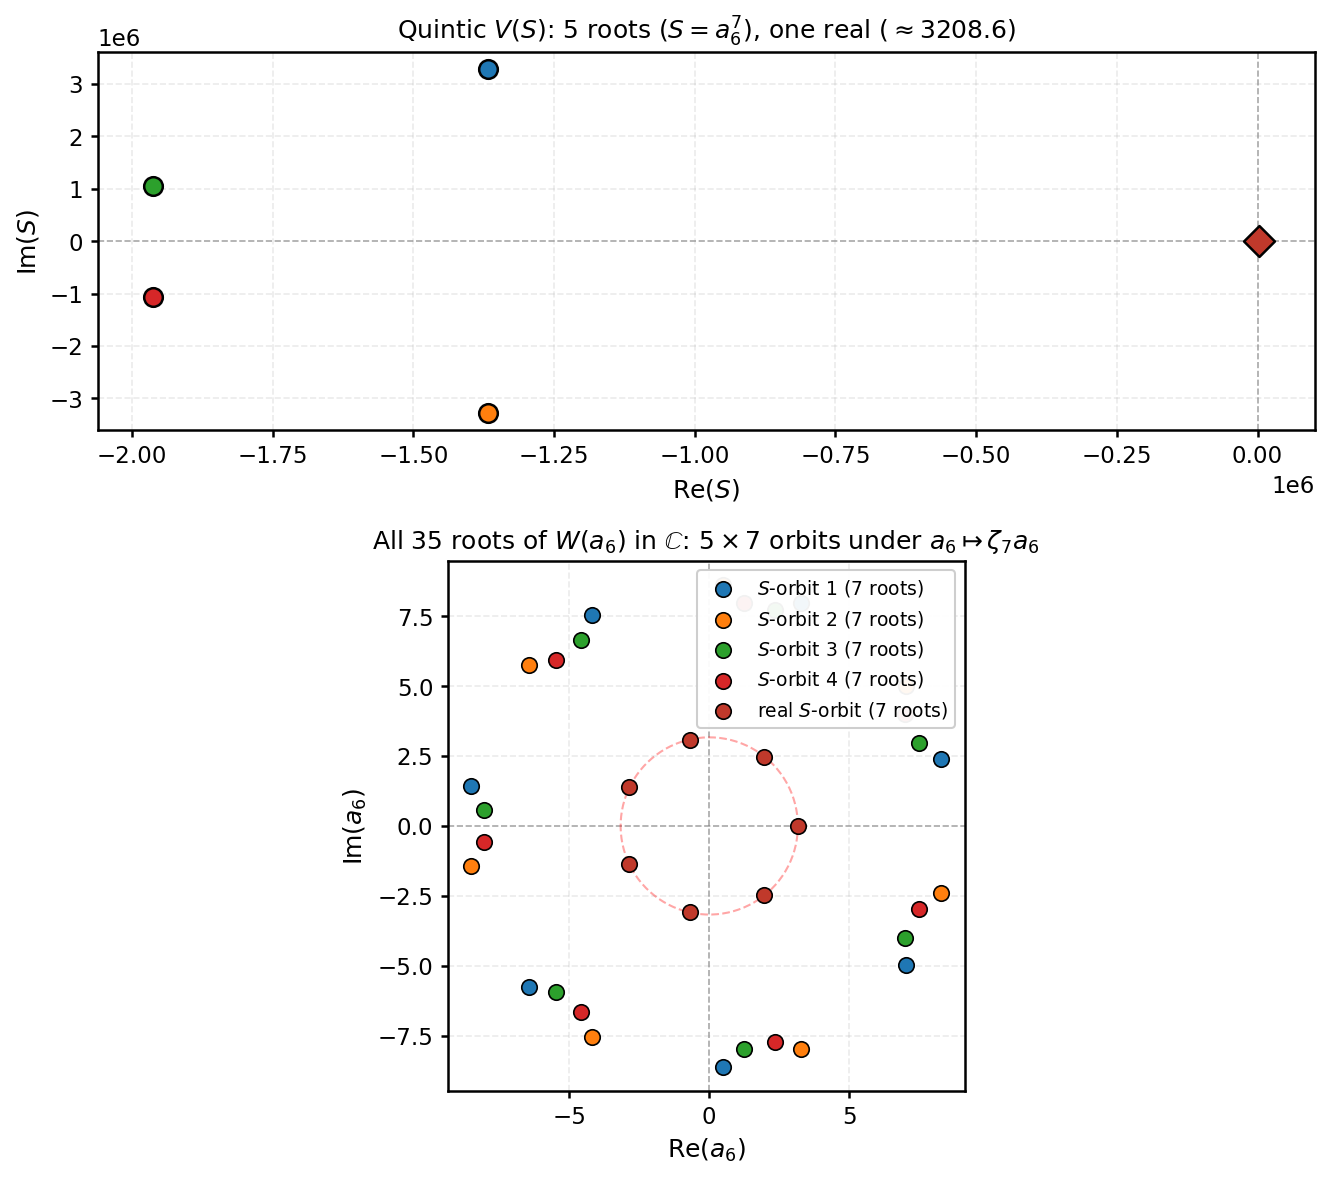
\includegraphics[width=0.85\linewidth]{figures/fig3_top_layer.png}
\caption{Top: the five roots of the quintic $V(S)$ in the complex $S$-plane, computed from the integer coefficients; the real root $S\approx3208.61$ is marked with a diamond. Bottom: all $35$ roots of $\mathcal{W}(a_6)$ in $\mathbb{C}$, colored by $S$-orbit; each $S\neq0$ lifts to $7$ values of $a_6$ via $7$th roots of unity. The dashed circle marks the real $S$-orbit. The $35$ roots form a single Galois orbit over $\mathbb{Q}$.}
\label{fig:top}
\end{figure}

\begin{proof}
(i) Direct factorization in {\sc Singular} over $\mathbb{Q}$. (ii) By inspection: every exponent of $\mathcal{W}$ is divisible by $7$. (iii) Discriminant computed exactly in {\sc SymPy} (nonzero integer); real-root count via Sturm sequence gives exactly one real $S$. (iv) Direct $\gcd$ computation in $\mathbb{F}_{101}[a_6]$.
\end{proof}

\begin{remark}[Characteristic-zero/modular consistency]
Reducing the integer quintic $V$ modulo $101$ gives $58$ times the quintic obtained directly from the mod-$101$ Gr\"obner computation (equivalently, the mod-$101$ quintic is $54$ times $V$), confirming consistency between the characteristic-zero and modular routes.
\end{remark}


\subsection{An algebraic proof of the top-layer classification for $m=7$, and its formalization}\label{sec:chartproof}

The proof of Proposition~\ref{prop:top-class} above rests on Riemann's existence theorem, which is not in Mathlib (at least not in the version pinned by the artifact). For $m=7$ we now give a second proof of the classification it provides, in the normalized chart of \S\ref{sec:normalization}: every solution is one of the points $(P_j(w),Q_k(w))$ with $R(w)=0$, the five $K_5$-conjugates. This is the form in which the main theorem uses Proposition~\ref{prop:top-class}. The eliminant $\mathcal{W}$ and the cases $m=3,5$ are not reproved here. The proof is purely algebraic and valid over every field of characteristic~$0$, and it is formalized: Theorem~\ref{thm:chartclass} is the Lean theorem \texttt{chartClassification\_holds} (listing~\ref{lst:proofchartclass}). We work in the Lean chart of \S\ref{sec:normalization}: $\alpha=1+a_1u+\dots+a_7u^7$, $\beta=b_0+b_1u+\dots+b_9u^9+u^{10}$, and $E_n=\sum_{i+k=n}(1+2k-3i)\,a_ib_k$ ($1\le n\le 16$) is the coefficient of $u^n$ in $\alpha\beta+u(2\alpha\beta'-3\alpha'\beta)$.

\begin{theorem}[\texttt{chartClassification\_holds}]\label{thm:chartclass}
Let $L$ be a field of characteristic~$0$. Suppose $(a_1,\dots,a_7,b_0,\dots,b_9)\in L^{17}$ satisfies $E_1=\dots=E_{16}=0$ and $a_7^3b_0^2=1$. Then $(a_j,b_k)=(P_j(w),Q_k(w))$ for a root $w\in L$ of $R$. Here $P_j,Q_k\in\mathbb{Q}[w]$ are the coordinates in listing~\ref{lst:def-chartclass}.
\end{theorem}

\begin{proof}
\emph{Step 1: reversed coordinates.} Since $a_7^3b_0^2=1$, we have $a_7\neq0$. Put $y_i=a_{7-i}/a_7$ for $1\le i\le 6$ and $y_7=1/a_7$, and give $y_i$ the weight~$i$. Define $S_k\in\mathbb{Q}[y_1,\dots,y_7]$, weighted homogeneous of weight~$k$, by
\[
(1+y_1v+\dots+y_7v^7)^{3/2}=\sum_{k\ge0}S_k\,v^k ,
\]
or, equivalently, by $S_0=1$ and $2k\,S_k=\sum_{i=1}^{7}(5i-2k)\,y_i\,S_{k-i}$. Write $\tilde\beta_k=b_{10-k}$ for $0\le k\le 10$ (so $\tilde\beta_0=1$) and $\tilde\beta_k=0$ for $k>10$; in both recursions, terms with a negative index are zero. Reindexing $E_{17-k}$ by $i\mapsto 7-i$, $k\mapsto 10-k$ gives
\[
E_{17-k}/a_7=-2k\,\tilde\beta_k+\sum_{i=1}^{7}(5i-2k)\,y_i\,\tilde\beta_{k-i}\qquad(1\le k\le 16).
\]
This is the recursion for $S_k$. Induction on $k$ gives $b_{10-k}=S_k(y)$ for $1\le k\le 10$, and
\begin{equation}\label{eq:Ssystem}
S_{11}(y)=\dots=S_{16}(y)=0,\qquad S_{10}(y)^2=y_7^3 .
\end{equation}
The last equation holds because $b_0=S_{10}(y)$ and $a_7^3b_0^2=1$. In the language of \S\ref{sec:top}, the reversed $\beta$ is the truncation of the power-series square root of the reversed $\alpha^3/a_7^3$. This is the Davenport--Stothers condition.

\emph{Step 2: the orbit relations.} Consider the six weighted-homogeneous relations
\begin{align*}
y_4&=\tfrac{2431}{18240}y_1^4-\tfrac{1027}{1710}y_1^2y_2+\tfrac{143}{380}y_2^2+\tfrac{41}{60}y_1y_3,\\
y_5&=\tfrac{1154351}{25313472}y_1^5-\tfrac{3833107}{18985104}y_1^3y_2+\tfrac{6512}{43947}y_1y_2^2+\tfrac{24449}{166536}y_1^2y_3,\\
y_6&=\tfrac{4206749569}{4242031637760}y_1^6+\tfrac{8589189473}{1590761864160}y_1^4y_2-\tfrac{440013827}{9819517680}y_1^2y_2^2\\&\qquad+\tfrac{7454351}{734423760}y_1^3y_3+\tfrac{253}{5054}y_2^3,\\
y_7&=-\tfrac{4539711243127}{16353031963564800}y_1^7+\tfrac{13373800868041}{6132386986336800}y_1^5y_2-\tfrac{214713769679}{37854240656400}y_1^3y_2^2\\&\qquad+\tfrac{81661753}{707800898700}y_1^4y_3+\tfrac{92333}{19483170}y_1y_2^3,\\
y_2y_3&=\tfrac{3738317}{46630080}y_1^5-\tfrac{16882087}{34972560}y_1^3y_2+\tfrac{115021}{161910}y_1y_2^2+\tfrac{2277881}{5828760}y_1^2y_3,\\
y_3^2&=\tfrac{740761013029}{10605079094400}y_1^6-\tfrac{754440973541}{1988452330200}y_1^4y_2+\tfrac{3827878261}{8182931400}y_1^2y_2^2\\&\qquad+\tfrac{137816863}{918029700}y_1^3y_3+\tfrac{289}{12635}y_2^3 .
\end{align*}
Write $g=0$ for any of them. Each satisfies
\[
y_7^3\cdot g\in(S_{11},\dots,S_{16})\subset\mathbb{Q}[y_1,\dots,y_7],
\]
with explicit cofactors of $341$ to $694$ terms, whose numerators and denominators have at most $42$ digits. Since $y_7\neq0$, every solution of~\eqref{eq:Ssystem} satisfies all six relations.

The relations were found by exact interpolation on the $K_5$ point, as all weighted-homogeneous forms of weight at most~$7$ that vanish on the five orbits. The cofactors come from exact weighted-homogeneous linear algebra over $\mathbb{Q}$. Let $(g)$ be the ideal of the six relations. A Gr\"obner computation over $\mathbb{Q}$ (\filename{saturation\_check.py}) shows that $(S_{11},\dots,S_{16})\subseteq(g)$ and $(g):y_7=(g)$. With the certificates this gives
\[
(S_{11},\dots,S_{16}):y_7^\infty=(S_{11},\dots,S_{16}):y_7^3=(g).
\]
The ideal $(g)$ has Krull dimension~$1$ and needs all six generators, so it is a weighted complete intersection. It has exactly five solutions in the chart $y_1=1$ and none with $y_1=0$ other than $y=0$, in agreement with weighted B\'ezout, $4\cdot5\cdot5\cdot6\cdot6\cdot7/7!=5$. These facts explain the choice of relations but are not used in the proof.

\emph{Step 3: a resultant.} The relation for $y_7$ shows $y_7\in y_1\,\mathbb{Q}[y_1,y_2,y_3]$, so $y_1\neq0$. Put $t=y_2/y_1^2$ and $s=y_3/y_1^3$. The relation for $y_2y_3$ becomes $(t-c)\,s=N(t)$ with $c=\tfrac{2277881}{5828760}$ and $\deg N=2$, and the relation for $y_3^2$ becomes monic quadratic in~$s$. Their Sylvester resultant in $s$ is $\kappa\,m(t)$ with $\kappa\in\mathbb{Q}^\times$ and
\[
\begin{aligned}
m(t)={}&287548593020928\,t^5-688401965085696\,t^4+640652914818432\,t^3\\
&-292066554895024\,t^2+65563255857792\,t-5817852446211,
\end{aligned}
\]
which is irreducible over $\mathbb{Q}$. Hence $t-c$ is invertible modulo~$m$, and $s=q_3(t)$. The first four relations then give $y_i/y_1^i=q_i(t)$ for $4\le i\le 7$, with $q_i\in\mathbb{Q}[t]$ reduced modulo~$m$.

\emph{Step 4: the torus.} Let $z=1/y_1$. By weighted homogeneity,
\[
z^{10}S_{10}(y)=S_{10}\bigl(1,t,q_3(t),\dots,q_7(t)\bigr)\equiv\sigma(t)\pmod m\qquad\text{and}\qquad z^7y_7=q_7(t).
\] Multiplying $S_{10}^2=y_7^3$ by $z^{21}$ gives $z\,\sigma(t)^2=q_7(t)^3$, that is,
\[
y_1=\sigma(t)^2\,q_7(t)^{-3}\bmod m(t).
\]
This fixes the torus without a seventh root, as in \S\ref{sec:normalization}, and makes every $y_i$ a polynomial in $t$ modulo~$m$. The substitution $w=\omega(t)$, with $\omega\in\mathbb{Q}[t]$ of degree~$4$, induces an isomorphism $\mathbb{Q}[t]/(m)\cong\mathbb{Q}[w]/(R)=K_5$ and gives $R(w)=0$ and $y_i=Y_i(w)$.

\emph{Step 5: back to the chart.} The formulas $a_7=1/y_7$ and $a_{7-i}=y_i/y_7$, together with the recursion of Step~1 for $b_{10-k}$, give $a_j=P_j(w)$ and $b_k=Q_k(w)$.
\end{proof}

\begin{lemma}[Characteristic-zero transfer]\label{lem:chart-transfer}
Let $F$ be a field of characteristic~$0$. Every $F$-valued solution of the normalized $m=7$ chart system is obtained by specializing the $K_5$-point at a root $w\in F$ of $R$; its five specializations at the five roots of $R$ (over a splitting field of $R$) are the five solutions.
\end{lemma}
\begin{proof}
Steps~1--5 are proved algebraically over $\mathbb{Q}$ and hence hold over every characteristic-zero field by base change. The Lean formalization quantifies over all $L$ with \texttt{CharZero}. The five solutions are the $K_5$-conjugates $(P_j(w),Q_k(w))$ with $R(w)=0$.
\end{proof}

\begin{remark}[Roles of the two classifications]
The $m=7$ case of Proposition~\ref{prop:top-class} is proved twice. The Belyi route combines the geometric upper bound (at most $35$ chart points over $\mathbb{C}$) with the $35$ exhibited points from the msolve parametrization, giving a complete classification in characteristic~$0$; it depends on Riemann's existence theorem and the computed parametrization. The algebraic certificate of this section gives an independent classification: every solution in characteristic~$0$ is one of the five $K_5$-orbits (Lemma~\ref{lem:chart-transfer}). Lean's \texttt{main\_theorem} uses only the algebraic route.
\end{remark}

\begin{remark}[Formalization]\label{rem:chartproof-lean}
The proof is formalized in \filename{lean/Jacobian/ChartProof/}: $12$ modules, all generated by \filename{lean/certgen/chartproof/} except the hand-written \filename{Reflect.lean}.
\begin{itemize}[nosep]
\item \emph{Steps.} There are $111$ steps. In $105$ of them a polynomial $g$ vanishes because $g=\sum_i c_ie_i$ for polynomials $e_i$ already known to vanish. In the other six, one for each relation of Step~2, the identity $y_7^3\,g=e$ holds with $e$ already known to vanish, and $y_7^3$ is cancelled using $y_7\neq0$.
\item \emph{Kernel checking.} Every identity is checked by the Lean kernel. \texttt{lc\_zero} (listing~\ref{lst:lczero}) and \texttt{eq\_of\_toPolyK} reduce it to an equality of normal forms. These are computed by the verified normalizer of \texttt{Lean.Grind.CommRing} from Lean core, with a kernel-friendly multiplication defined by recursors (\texttt{toPolyK}, soundness theorem \texttt{denote\_toPolyK}), and \texttt{decide +kernel} evaluates them.
\item \emph{Axioms.} No \texttt{native\_decide} is used. \texttt{\#print axioms} for \texttt{chartClassification\_holds} and for \texttt{main\_theorem} reports only \texttt{propext}, \texttt{Classical.choice} and \texttt{Quot.sound}.
\item \emph{Batching.} The certificates of Step~2 have between $27{,}747$ and $56{,}999$ monomial products each. They are split into batches of at most $9{,}000$ products, one declaration per batch.
\item \emph{Independent checks.} Every certificate was also verified by exact SymPy expansion before it was written, and the generator reproduces all eleven generated modules byte-identically. A second checker, written independently of the generator (\filename{independent\_check.py}), parses the Lean text and re-verifies all $111$ identities over $\mathbb{Z}$. This checker verifies the arithmetic of the certificates only; it does not re-prove the mathematical statements. The Lean kernel remains solely responsible for verifying that these certificates prove the stated formal propositions. Six controls behave as expected: four one-integer perturbations are rejected by \texttt{decide}, a planted \texttt{sorry} is flagged, and an unmodified module is accepted.
\item \emph{Cost.} The build takes about $25$ minutes sequentially and needs at most $5.4$\,GB of memory for any one module.
\end{itemize}
\end{remark}

\begin{remark}[Why these coordinates]
Earlier formulations failed to yield certificates of practical size because of the degenerate Davenport--Stothers components of lower degree (the solutions for $m=1,3,5$). With $a_0=b_0=1$ and $b$ eliminated, these components force saturation by $a_7^7$ or $a_7^8$, so the certificates have weight~$61$. In the chart $a_0=b_{10}=1$, the sub-case $a_1=0$ alone needed $503{,}254$ cofactor terms modulo a prime. Replayed over~$\mathbb{Q}$, its Buchberger trace reached coefficients of $2{,}722$ digits after $929$ of its $2{,}065$ elements (\filename{lean/CLASSIFICATION\_STATUS.md}, \S5). In the reversed coordinates the same components lie on $y_7=0$, and $y_7^3$ suffices, at weight at most~$28$. The five orbits then form a weighted complete intersection that can be written down explicitly. The six certificates of Step~2 have $341$ to $694$ cofactor terms each over~$\mathbb{Q}$, roughly a thousand times fewer than the modular lift for $a_1=0$ alone.
\end{remark}

% keep the caption of the next listing on the same page as its code
\par\vskip 0pt plus 8\baselineskip\penalty-200\vskip 0pt plus -8\baselineskip\relax
% BEGIN-MECHANICAL:lst:proofchartclass
\begin{leanlisting}{Mechanically extracted from \texttt{Jacobian/ChartProof/Final.lean} (sha256 \texttt{638b644ffb58cb8b}); statement verbatim, proof elided.}{lst:proofchartclass}
theorem chartClassification_holds (L : Type*) [Field L] [CharZero L] : ChartClassification L := by
  -- proof body elided (see artifact)
\end{leanlisting}
% END-MECHANICAL:lst:proofchartclass
% BEGIN-MECHANICAL:lst:unconditional
\begin{leanlisting}{Mechanically extracted from \texttt{Jacobian/ChartProof/Final.lean} (sha256 \texttt{638b644ffb58cb8b}); statement verbatim, proof elided.}{lst:unconditional}
theorem main_theorem {L : Type*} [Field L] [CharZero L] :
    ¬ ∃ (P Q : MvPolynomial (Fin 2) L) (lam : L), lam ≠ 0 ∧ NewtonNF2 P Q ∧ jac P Q = MvPolynomial.C lam * MvPolynomial.X 0 ^ 2 :=
  -- proof term elided (see artifact)
\end{leanlisting}
% END-MECHANICAL:lst:unconditional
% BEGIN-MECHANICAL:lst:lczero
\begin{leanlisting}{Mechanically extracted from \texttt{Jacobian/ChartProof/Reflect.lean} (sha256 \texttt{9e3ea428ffe7236b}); statement verbatim, proof elided.}{lst:lczero}
theorem lc_zero (ctx : Context α) (g : Expr) (l : List (Expr × Expr))
    (hcert : Poly.beq' (toPolyK (.sub g (lcExpr l))) (.num 0) = true) (h : AllZero ctx l) :
    g.denote ctx = 0 := by
  -- proof body elided (see artifact)
\end{leanlisting}
% END-MECHANICAL:lst:lczero

\section{Descent}\label{sec:descent}

Fix a top-layer solution $(\alpha,\beta)$. The descent solves $E_4,E_3,E_2$ in turn. We use the scaled variables $A_2=u\alpha$ and $B_3=u^2\beta$.

\subsection{\texorpdfstring{Layer $E_4$}{Layer E4}}

\begin{proposition}[$E_4$ structure]\label{prop:e4}
$E_4$ is a linear system in $19$ unknowns ($A_1$ on $u^1,\dots,u^8$; $B_2$ on $u^2,\dots,u^{12}$) with $18$ equations, rank $17$, and kernel dimension $2$. The kernel is parametrized by $t=(t_1,t_2)$, giving $(A_1(t),B_2(t))$ linear in $t$. Computed exactly in characteristic zero over the quintic field $K_5=\mathbb{Q}[w]/(w^5-w^4+3w^3+3w^2+26)$ (script \filename{exact\_ranks\_K5.py}); the modular evaluation at $p=101$, $a_6=55$ is an independent cross-check.
\end{proposition}

\begin{proof}
Rank computation on the $18\times19$ coefficient matrix, with residual asserts verifying the kernel. Scripts: \filename{exact\_ranks\_K5.py} (exact rank and kernel over $K_5$) and \filename{C5\_E2\_obstruction\_corrected.py} (which verifies $E_4$ with $E_4$-kernel residuals zero; mod-$101$ cross-check).
\end{proof}

\subsection{\texorpdfstring{Layer $E_3$}{Layer E3}}

\begin{proposition}[$E_3$ structure and unconditional solvability]\label{prop:e3}
$E_3$ is a $19\times20$ linear system of rank $18$ with $2$-dimensional kernel. Moreover, $E_3$ is solvable for \emph{every} direction $t=(t_1,t_2)$: writing the system as $M(t)x=K(t)$ with $M$ constant and $K$ quadratic in $t$, the left nullvector $v$ (with $v^\top M=0$) satisfies
\begin{equation}
v^\top K_{11}\equiv0,\qquad v^\top K_{22}\equiv0,\qquad v^\top K_{12}\equiv0
\end{equation}
identically as polynomials in $t$, where $K=t_1^2K_{11}+t_1t_2K_{12}+t_2^2K_{22}$. Hence no direction is obstructed at $E_3$. All computations are exact over $K_5$; see Lemma~\ref{lem:lifting}(i).
\end{proposition}

\begin{proof}
The $19\times20$ matrix $M$ has rank $18$; its left nullspace is $1$-dimensional, spanned by $v$. Decomposing the inhomogeneous part and computing $v^\top K_{ij}$ symbolically gives zero for all $i,j$. Script: \filename{C5\_E2\_obstruction\_corrected.py} (which verifies $E_3$ with residual asserts).
\end{proof}

The general solution of $E_3$ is thus the $2$-parameter affine family
\begin{equation}
x(t,s)=t_1^2x_{11}+t_1t_2x_{12}+t_2^2x_{22}+s_1w_1+s_2w_2,
\end{equation}
encoding $(A_0,B_1)$ in terms of $(t,s)=(t_1,t_2,s_1,s_2)\in\mathbb{C}^4$.

\subsection{\texorpdfstring{Layer $E_2$}{Layer E2}}

\begin{proposition}[$E_2$ injectivity]\label{prop:e2}
The homogeneous operator of $E_2$ in the unknown $B_0'$ is a $19\times12$ matrix of rank $12$, hence injective. Its left nullspace has dimension $19-12=7$. Exact over $K_5$; see Lemma~\ref{lem:lifting}(i)--(ii).
\end{proposition}

Therefore $B_0'$ (and hence $B_0$ up to an additive constant) is uniquely fixed by $(A_0,B_1,A_1,B_2)$. The seven left-nullvector pairings then give seven compatibility conditions:
\begin{equation}\label{eq:seven}
W\cdot\mathrm{rhs}(t,s)=0,
\end{equation}
where $W$ is $7\times19$ and $\mathrm{rhs}(t,s)$ is the $E_2$ inhomogeneous term. These seven conditions are the \emph{only} remaining obstructions; $E_1$ is never needed.

% BEGIN-MECHANICAL:lst:descent
\begin{leanlisting}{Mechanically extracted from \texttt{Jacobian/Descent/Main.lean} (sha256 \texttt{e18a3a9e531df6d6}); statement verbatim, proof elided.}{lst:descent}
theorem descent_K5 {L : Type*} [Field L] [CharZero L]
    (w : L)
    (hw : w ^ 5 - w ^ 4 + 3 * w ^ 3 + 3 * w ^ 2 + 26 = 0)
    (a_1_0 a_2_2 a_3_4 a_4_6 a_5_8 a_6_10 a_7_12 a_8_14 b_2_1 b_3_3 b_4_5 b_5_7 b_6_9 b_7_11 b_8_13 b_9_15 b_10_17 b_11_19 b_12_21 : L)
    (h_a_1_0 : a_1_0 = ((1 : L)))
    -- ... (18 h4_*, 19 h3_*, 19 h2_*, 8 h_a_*, 11 h_b_*, 51 lower-layer unknowns in one binder)
    (hv : b_12_24 ≠ 0) :
    False := by
  -- proof body elided (see artifact)
\end{leanlisting}
% END-MECHANICAL:lst:descent

\section{The final obstruction}\label{sec:obstruction}

We use the homogeneous formulation: $E_3$ with $A_0$ on $u^1,\dots,u^8$ ($a_{8,16}$ free, no constant term) and $B_1$ on $u^1,\dots,u^{12}$. This gives the genuine $2$-dimensional kernel with two independent directions $s=(s_1,s_2)$, both moving actual coefficients. (An earlier formulation froze $a_{8,16}=1$ and included the constant term as an unknown; the constant is killed by $A_0'$ and contributes only a trivial direction.)

\begin{remark}[Free parameter]
\S\ref{sec:normalization} leaves $a_{8,16}$ free from the start. The $E_2$/$E_3$ analysis therefore applies to every slice, including $a_{8,16}=1$, without a superset argument.
\end{remark}

\subsection{Explicit form of the seven conditions}

Expanding~\eqref{eq:seven} symbolically in $(t_1,t_2,s_1,s_2)$ gives:

\begin{lemma}\label{lem:seven-explicit}
Each of the seven conditions has the form
\begin{equation}
b_i(t_1,t_2)+s_1\cdot M_i(t_1,t_2)+s_2\cdot L_i(t_1,t_2)=0,\qquad i=1,\dots,7,
\end{equation}
where $b_i$ is homogeneous cubic and $M_i,L_i$ are linear in $(t_1,t_2)$. Both $s_1$ and $s_2$ appear genuinely.
\end{lemma}

\begin{proof}
Exact expansion over $K_5$ in python-flint (script \filename{exact\_obstruction\_K5.py}) of $W\cdot\mathrm{rhs}(t,s)$ with the homogeneous $E_3$ parametrization $x(t,s)=t_1^2x_{11}+t_1t_2x_{12}+t_2^2x_{22}+s_1w_1+s_2w_2$ substituted; the {\sc SymPy} expansion over $\mathbb{F}_{101}$ (script \filename{C5\_E2\_obstruction\_corrected.py}) is a cross-check.
\end{proof}

\subsection{\texorpdfstring{Elimination of $(s_1,s_2)$}{Elimination of (s1,s2)}}

For fixed $t\neq0$, the seven equations are affine-linear in $(s_1,s_2)$. A solution can exist only if the $7\times3$ matrix $[b(t)\mid M(t)\mid L(t)]$ has rank at most $2$, i.e.\ only if all $3\times3$ minors vanish:
\begin{equation}\label{eq:minors}
\det\begin{pmatrix}
b_i & M_i & L_i \\ b_j & M_j & L_j \\ b_k & M_k & L_k
\end{pmatrix}=0,\qquad 1\leq i<j<k\leq7.
\end{equation}
There are $\binom{7}{3}=35$ such minors, each a homogeneous binary quintic in $(t_1,t_2)$ (cubic $\times$ linear $\times$ linear).

\begin{theorem}[No nonzero direction]\label{thm:no-direction}
The $35$ quintics~\eqref{eq:minors} span the degree-five homogeneous component $K_5[t_1,t_2]_5$ and generate the ideal $(t_1,t_2)^5$, i.e.\ they have Gr\"obner basis
\begin{equation}
(t_1,t_2)^5 = \left\{\, t_1^5,\; t_1^4 t_2,\; t_1^3 t_2^2,\; t_1^2 t_2^3,\; t_1 t_2^4,\; t_2^5 \,\right\}
\end{equation}
exactly over $K_5$ (the $35\times6$ coefficient matrix has rank $6$, spanning all binary quintics). Hence their common projective zero locus is empty and their only common affine zero in $\overline{K_5}^2$ is $(0,0)$: there is \emph{no} nonzero $t$ admitting $(s_1,s_2)$ satisfying the seven $E_2$ conditions. The mod-$101$ Gr\"obner computation (lex order) is an independent cross-check.
\end{theorem}

\begin{proof}
Exact computation over $K_5$: the $35$ minors are homogeneous quintics, and their $35\times6$ coefficient matrix has rank~$6$, so
\[
\operatorname{span}_{K_5}\{M_{ijk}\}=K_5[t_1,t_2]_5,
\]
the full six-dimensional space of binary quintics. Hence every degree-five monomial lies in the ideal $I$ they generate, i.e.\ $(t_1,t_2)^5\subseteq I$; conversely each generator lies in $(t_1,t_2)^5$, so $I=(t_1,t_2)^5$. The radical is $(t_1,t_2)$, so the affine variety over the algebraic closure is $\{(0,0)\}$. Script: \filename{exact\_obstruction\_K5.py}, which also writes the $35\times6$ matrix and a $6\times6$ nonzero minor to \filename{logs/k5\_minor\_certificate.json} as a machine-readable certificate. The {\sc SymPy} Gr\"obner basis over $GF(101)$ (script \filename{C5\_E2\_obstruction\_corrected.py}, saved, rerunnable; log archived) is a cross-check.
\end{proof}

\begin{remark}[Interpretation]
The top layer admits five characteristic-zero orbits, but none extends to a full solution: the $E_4$ kernel gives a two-dimensional space of directions $t\in K^2$, the $E_3$ layer imposes no further restriction, and then the seven $E_2$ compatibility conditions force $t=0$ via the $35$ quintic minors. The remaining case $t=0$ is ruled out separately (Corollary~\ref{cor:t0}). In other words, the top-layer solutions exist in isolation, but none extends to a Newton-normal-form pair with $[P,Q]=\lambda x^2$.
\end{remark}

\subsection{\texorpdfstring{The case $t=0$}{The case t=0}}

\begin{lemma}[Collapse at $t=0$]\label{lem:t0-collapse}
At $t=(0,0)$ the $E_2$ layer equation reduces to
\[
2A_2B_0'=0.
\]
\end{lemma}
\begin{proof}
Because the target bracket identity $[P,Q]=x^2=u^2y^{-4}$ contains only a $y^{-4}$ component, the layer equation $E_4$ at $y^{-3}$ is homogeneous:
\[
2(A_2B_2'-A_2'B_2)+(A_1B_3'-3A_1'B_3)=0.
\]
Consequently $t=(0,0)$ forces $(A_1,B_2)\equiv(0,0)$. In layer $E_3$ the quadratic driving term $K(t)$ vanishes identically at $t=0$, leaving only the homogeneous kernel. In layer $E_2$ the terms $(A_1B_1'-A_1'B_1)-2A_0'B_2$ then vanish identically, leaving $2A_2B_0'=0$.
\end{proof}

\begin{corollary}[$t=0$ impossible]\label{cor:t0}
By Lemma~\ref{lem:t0-collapse}, at $t=0$ we have $2A_2B_0'=0$. Since $A_2=u\alpha\neq0$, this requires $B_0'=0$, forcing $B_0(u)$ to be constant. Hence $b_{12,24}=0$; in particular, $(12,24)$ cannot be a vertex of $N(Q)$.
\end{corollary}

\begin{remark}
The Lean formalization \texttt{e2\_t0} (listing~\ref{lst:t0}) proves $b_{12,24}=0$ via a \emph{different route}: a left-inverse certificate on the reduced $E_2$ equations with $t=0$ supplied as hypotheses, rather than the $2A_2B_0'=0$ argument above. Both routes reach the same conclusion.
\end{remark}

% BEGIN-MECHANICAL:lst:t0
\begin{leanlisting}{Mechanically extracted from \texttt{Jacobian/Descent/E2/T0.lean} (sha256 \texttt{3559bcbdbff42d3c}); statement verbatim, proof elided.}{lst:t0}
theorem e2_t0 {L : Type*} [Field L] [CharZero L]
    (w : L)
    (hw : w ^ 5 - w ^ 4 + 3 * w ^ 3 + 3 * w ^ 2 + 26 = 0)
    (b_11_20 b_12_22 b_11_21 b_12_23 b_1_2 b_2_4 b_3_6 b_4_8 b_5_10 b_6_12 b_7_14 b_8_16 b_9_18 b_10_20 b_11_22 b_12_24 : L)
    -- 19 reduced E2 equations (r2_1_1) ... (r2_19_37), hypotheses elided for brevity
    (ht1 : b_11_20 = 0)
    (ht2 : b_12_22 = 0) :
    b_12_24 = 0 := by
  -- proof body elided (see artifact)
\end{leanlisting}
% END-MECHANICAL:lst:t0

\subsection{Proof of the main theorem}

\begin{proof}[Proof of Theorem~\ref{thm:main}]
By Proposition~\ref{prop:layers}, the layers satisfy $E_5,\dots,E_1$. Since $a_{1,0}\cdot a_{8,14}\cdot b_{2,1}\cdot b_{12,21}\neq 0$, Proposition~6.1 puts $(A_2,B_3)$ in the torus orbit of the $K_5$ point for some root $w$ of $R$. By torus transport (Listing~\ref{lst:torus}) we may take it to be that point. Propositions~\ref{prop:e4}--\ref{prop:e2} and Theorem~\ref{thm:no-direction} force $t=0$. At $t=0$, Lemma~\ref{lem:t0-collapse} and Corollary~\ref{cor:t0} give $B_0'=0$, so $b_{12,24}=0$ (in Lean, \texttt{e2\_t0}, Listing~\ref{lst:t0}). The last sentence of the theorem follows because $\mathrm{NewtonNF2}$ requires $b_{12,24}\neq 0$.
\end{proof}

\begin{proof}[Proof of Corollary~\ref{cor:a816}]
At the $K_5$ point, let $e_1,\dots,e_{75}$ be the coefficients of $[P,Q]-x^2$ in the layers $E_4,\dots,E_1$, as built by \filename{scripts/a816\_full.sing}; their unknowns are the $51$ lower coefficients of $P$ and $Q$ that occur. There is an explicit identity
\[
a_{8,16}^2=\sum_{k=1}^{75}H_k\,e_k,\qquad H_k\in K_5[a,b],
\]
stored in Rabinowitsch form, $1=\sum_k z^2H_k\,e_k-(1+a_{8,16}z)(a_{8,16}z-1)$, as the $76$ cofactors of \filename{scripts/a816\_certificate/a816\_lift.txt} ($3464$ terms, coefficients of at most $493$ digits). It is built from the layer structure. Give the coefficients of $A_1,B_2$ depth~$1$, those of $A_0,B_1$ depth~$2$ and those of $B_0$ depth~$3$; each equation of $E_{5-d}$ is then homogeneous of depth~$d$ and linear in the unknowns of depth~$d$. Row reduction of these linear parts in $E_4$, $E_3$, $E_2$ (ranks $17$, $18$, $12$ over $K_5$) expresses every unknown, modulo the layer ideal, as a polynomial in four free ones, $\tau=(b_{11,20},b_{12,22})$ of depth~$1$ and $\sigma=(a_{8,16},b_{11,21})$ of depth~$2$. The $32$ products of depth~$4$ formed from the reduced generators span all $14$ monomials of depth~$4$ in $K_5[\tau,\sigma]$, and lifting back gives the $H_k$. The identity is checked exactly by {\sc Singular} over $\mathbb{Q}(w)$ and independently by python-flint, which rebuilds $[P,Q]$ from $P$ and $Q$ (\filename{scripts/a816\_certificate/verify\_bundle.sh}). Hence $a_{8,16}=0$ at the $K_5$ point once $E_1$ is included. Torus transport multiplies $a_{8,16}$ by a nonzero scalar, so $a_{8,16}=0$ on the whole orbit.
\end{proof}

\begin{remark}[Further rigidity, outside the certificate]\label{rem:full-rigidity}
The same span statement puts every monomial of depth at least~$4$ in $\tau,\sigma$ into the layer ideal, so each of the $51$ unknowns (the non-constant lower coefficients of $P$ and $Q$) is nilpotent modulo it: at the $K_5$ point the only solution of $E_4,\dots,E_1$ is $P=P_2+\mathrm{const}$, $Q=Q_3+\mathrm{const}$. This stronger statement rests on one exact rank computation over $K_5$ (\filename{scripts/a816\_certificate/structured\_cert.py}), corroborated modulo a prime; only the identity for $a_{8,16}$ is written out and checked twice. It is not used elsewhere.
\end{remark}

\begin{proof}[Proof of Corollary~\ref{cor:gghv}]
Proposition~4.3 of~\cite{GGHV}, then Theorem~\ref{thm:main}.
\end{proof}

% BEGIN-MECHANICAL:lst:main
\begin{leanlisting}{Mechanically extracted from \texttt{Jacobian/BranchAbFinal.lean} (sha256 \texttt{cd4e207adba5cb7b}); statement verbatim, proof elided.}{lst:main}
theorem no_completion_K5 {L : Type*} [Field L] [CharZero L] (w : L)
    (hw : w ^ 5 - w ^ 4 + 3 * w ^ 3 + 3 * w ^ 2 + 26 = 0) (lam : L)
    (A₀ A₁ A₂ B₀ B₁ B₂ B₃ : Polynomial L) (p₀ p₁ p₂ q₀ q₁ q₂ q₃ : MvPolynomial (Fin 2) L)
    (hp₀ : X 1 ^ 0 * p₀ = evH A₀) (hp₁ : X 1 ^ 1 * p₁ = evH A₁) (hp₂ : X 1 ^ 2 * p₂ = evH A₂)
    (hq₀ : X 1 ^ 0 * q₀ = evH B₀) (hq₁ : X 1 ^ 1 * q₁ = evH B₁) (hq₂ : X 1 ^ 2 * q₂ = evH B₂)
    (hq₃ : X 1 ^ 3 * q₃ = evH B₃)
    (hJ : jac (p₀ + p₁ + p₂) (q₀ + q₁ + q₂ + q₃) = C lam * X 0 ^ 2)
    (sA₀ : ∀ i, A₀.coeff i ≠ 0 → 0 ≤ i ∧ i ≤ 8)
    (sA₁ : ∀ i, A₁.coeff i ≠ 0 → 1 ≤ i ∧ i ≤ 8)
    (sA₂ : ∀ i, A₂.coeff i ≠ 0 → 1 ≤ i ∧ i ≤ 8)
    (sB₀ : ∀ i, B₀.coeff i ≠ 0 → 0 ≤ i ∧ i ≤ 12)
    (sB₁ : ∀ i, B₁.coeff i ≠ 0 → 1 ≤ i ∧ i ≤ 12)
    (sB₂ : ∀ i, B₂.coeff i ≠ 0 → 2 ≤ i ∧ i ≤ 12)
    (sB₃ : ∀ i, B₃.coeff i ≠ 0 → 2 ≤ i ∧ i ≤ 12)
    (ρ σ ε : L) (hρ : ρ ≠ 0) (hσ : σ ≠ 0) (hε : ε ≠ 0)
    (t_a_1_0 : (A₂.coeff 1) = ρ * ε ^ (0 : ℕ) * ((1 : L)))
    (t_a_2_2 : (A₂.coeff 2) = ρ * ε ^ (1 : ℕ) * (((303) / 16 : L) + ((879) / 128 : L) * w + ((-389) / 128 : L) * w ^ (2 : ℕ) + ((-51) / 128 : L) * w ^ (3 : ℕ) + ((49) / 128 : L) * w ^ (4 : ℕ)))
    (t_a_3_4 : (A₂.coeff 3) = ρ * ε ^ (2 : ℕ) * (((315) / 16 : L) + ((693) / 8 : L) * w + ((-147) / 8 : L) * w ^ (2 : ℕ) + ((-189) / 8 : L) * w ^ (3 : ℕ) + ((147) / 16 : L) * w ^ (4 : ℕ)))
    (t_a_4_6 : (A₂.coeff 4) = ρ * ε ^ (3 : ℕ) * (((-79653) / 64 : L) + ((29463) / 64 : L) * w + ((7371) / 128 : L) * w ^ (2 : ℕ) + ((-4767) / 16 : L) * w ^ (3 : ℕ) + ((8001) / 128 : L) * w ^ (4 : ℕ)))
    (t_a_5_8 : (A₂.coeff 5) = ρ * ε ^ (4 : ℕ) * (((-33519) / 4 : L) + ((-6843) / 4 : L) * w + ((8181) / 8 : L) * w ^ (2 : ℕ) + ((-1713) / 2 : L) * w ^ (3 : ℕ) + ((-1305) / 8 : L) * w ^ (4 : ℕ)))
    (t_a_6_10 : (A₂.coeff 6) = ρ * ε ^ (5 : ℕ) * (((-8805) / 8 : L) + ((-76965) / 8 : L) * w + ((11523) / 16 : L) * w ^ (2 : ℕ) + ((6927) / 4 : L) * w ^ (3 : ℕ) + ((-18579) / 16 : L) * w ^ (4 : ℕ)))
    (t_a_7_12 : (A₂.coeff 7) = ρ * ε ^ (6 : ℕ) * (((389740) / 17 : L) + ((-51922) / 17 : L) * w + ((-48572) / 17 : L) * w ^ (2 : ℕ) + ((63239) / 17 : L) * w ^ (3 : ℕ) + ((-6475) / 17 : L) * w ^ (4 : ℕ)))
    (t_a_8_14 : (A₂.coeff 8) = ρ * ε ^ (7 : ℕ) * (((476437) / 68 : L) + ((314405) / 68 : L) * w + ((-174571) / 136 : L) * w ^ (2 : ℕ) + ((1574) / 17 : L) * w ^ (3 : ℕ) + ((82783) / 136 : L) * w ^ (4 : ℕ)))
    (t_b_2_1 : (B₃.coeff 2) = σ * ε ^ (0 : ℕ) * ((1 : L)))
    (t_b_3_3 : (B₃.coeff 3) = σ * ε ^ (1 : ℕ) * (((101) / 8 : L) + ((293) / 64 : L) * w + ((-389) / 192 : L) * w ^ (2 : ℕ) + ((-17) / 64 : L) * w ^ (3 : ℕ) + ((49) / 192 : L) * w ^ (4 : ℕ)))
    (t_b_4_5 : (B₃.coeff 4) = σ * ε ^ (2 : ℕ) * (((315) / 16 : L) + ((693) / 8 : L) * w + ((-147) / 8 : L) * w ^ (2 : ℕ) + ((-189) / 8 : L) * w ^ (3 : ℕ) + ((147) / 16 : L) * w ^ (4 : ℕ)))
    (t_b_5_7 : (B₃.coeff 5) = σ * ε ^ (3 : ℕ) * (((-11379) / 8 : L) + ((4209) / 8 : L) * w + ((1053) / 16 : L) * w ^ (2 : ℕ) + ((-681) / 2 : L) * w ^ (3 : ℕ) + ((1143) / 16 : L) * w ^ (4 : ℕ)))
    (t_b_6_9 : (B₃.coeff 6) = σ * ε ^ (4 : ℕ) * (((-695299) / 48 : L) + ((-48367) / 48 : L) * w + ((52679) / 32 : L) * w ^ (2 : ℕ) + ((-45661) / 24 : L) * w ^ (3 : ℕ) + ((-2211) / 32 : L) * w ^ (4 : ℕ)))
    (t_b_7_11 : (B₃.coeff 7) = σ * ε ^ (5 : ℕ) * (((-309895) / 8 : L) + ((-251275) / 8 : L) * w + ((101481) / 16 : L) * w ^ (2 : ℕ) + ((1811) / 4 : L) * w ^ (3 : ℕ) + ((-60489) / 16 : L) * w ^ (4 : ℕ)))
    (t_b_8_13 : (B₃.coeff 8) = σ * ε ^ (6 : ℕ) * (((1733348) / 13 : L) + ((-2368725) / 26 : L) * w + ((-184976) / 13 : L) * w ^ (2 : ℕ) + ((1819939) / 52 : L) * w ^ (3 : ℕ) + ((-569071) / 52 : L) * w ^ (4 : ℕ)))
    (t_b_9_15 : (B₃.coeff 9) = σ * ε ^ (7 : ℕ) * (((18736247) / 39 : L) + ((1087133) / 13 : L) * w + ((-5656777) / 78 : L) * w ^ (2 : ℕ) + ((1993384) / 39 : L) * w ^ (3 : ℕ) + ((971365) / 78 : L) * w ^ (4 : ℕ)))
    (t_b_10_17 : (B₃.coeff 10) = σ * ε ^ (8 : ℕ) * (((305098) / 17 : L) + ((5784066) / 17 : L) * w + ((-308335) / 17 : L) * w ^ (2 : ℕ) + ((-950608) / 17 : L) * w ^ (3 : ℕ) + ((754021) / 17 : L) * w ^ (4 : ℕ)))
    (t_b_11_19 : (B₃.coeff 11) = σ * ε ^ (9 : ℕ) * (((-149721182) / 323 : L) + ((26391690) / 323 : L) * w + ((21560033) / 323 : L) * w ^ (2 : ℕ) + ((-24378412) / 323 : L) * w ^ (3 : ℕ) + ((2786935) / 323 : L) * w ^ (4 : ℕ)))
    (t_b_12_21 : (B₃.coeff 12) = σ * ε ^ (10 : ℕ) * (((-91912444) / 969 : L) + ((-20715500) / 323 : L) * w + ((17474146) / 969 : L) * w ^ (2 : ℕ) + ((-1623428) / 969 : L) * w ^ (3 : ℕ) + ((-8783302) / 969 : L) * w ^ (4 : ℕ)))
    (hv : B₀.coeff 12 ≠ 0) : False := by
  -- proof body elided (see artifact)
\end{leanlisting}
% END-MECHANICAL:lst:main

\section{Exact characteristic-\texorpdfstring{$0$}{0} descent}\label{sec:lifting}

The proof is exact over $K_5$ (items (i)--(ii) below).

\begin{lemma}[Base change for the $K_5$ computations]\label{lem:basechange}
$R(w)=w^5-w^4+3w^3+3w^2+26$ is irreducible and separable over $\mathbb{Q}$, so $K_5=\mathbb{Q}[w]/(R)$ is a number field. The coefficients of the $E_4,E_3,E_2$ matrices and of the seven compatibility polynomials lie in $K_5$. Exact rank identities and exact ideal identities over $K_5$ therefore remain valid under every characteristic-zero field extension.
\end{lemma}

\begin{proof}
$R$ is irreducible modulo $67$ (a single quintic factor), hence irreducible over $\mathbb{Q}$, and separable since its discriminant $784{,}822{,}272=2^{12}\cdot3\cdot13\cdot17^3$ is nonzero. Hence $K_5$ is a field. Rank of a matrix and equality of ideals are preserved under field extension: rank is the size of the largest nonzero minor, and ideal membership is witnessed by explicit polynomial combinations, both of which persist after extending scalars.
\end{proof}

\begin{lemma}[Exact obstruction]\label{lem:lifting}
Let $\rho\in\overline{\mathbb{Q}}$ be any root of $\mathcal{W}$, and put $K=\mathbb{Q}(\rho)$. The $E_2$ obstruction---no nonzero $(t_1,t_2)$ satisfies the seven compatibility conditions---holds over $K$.
\end{lemma}

\begin{proof}
By Lemma~\ref{lem:basechange}, the exact rank and ideal identities over $K_5$ persist under every characteristic-zero field extension. Since $K_5\cong\mathbb{Q}(\rho^7)$ for every root $\rho$ of $\mathcal{W}$ (the $S=a_6^7$ parametrization; Remark~\ref{rem:import}), the obstruction holds over $\mathbb{Q}(\rho)$, hence over every characteristic-zero field containing such a root. The ingredients are the exact characteristic-$0$ computations (scripts \filename{exact\_ranks\_K5.py}, \filename{exact\_obstruction\_K5.py}):
\begin{enumerate}[nosep]
\item[(i)] \emph{Exact characteristic-$0$ ranks.} The ranks are computed exactly over the quintic field $K_5=\mathbb{Q}[w]/(w^5-w^4+3w^3+3w^2+26)$ (script \filename{exact\_ranks\_K5.py}): $E_4=17$, $E_3=18$, $E_2=12$.
\item[(ii)] \emph{Exact descent over $K_5$.} The entire $E_4\to E_3\to E_2\to35$-minor pipeline is redone exactly over $K_5$ (script \filename{exact\_obstruction\_K5.py}, $\sim$1~s): $E_3$ is solvable for every $t$, the left nullity of $E_2$ is $7$, and the $35$ minors span \emph{all} binary quintics (the $35\times6$ coefficient matrix has rank~$6$ over $K_5$). Hence the only common zero is $t=0$. End-to-end residuals against the original bracket equations vanish exactly. The $t=0$ case is excluded by the vertex $(12,24)$ argument, which is valid in every characteristic other than $2$ and $3$ (it uses $2\ne0$ and $12\ne0$; see \S8.3). The Lean formalization (\texttt{no\_completion\_K5}, listing~\ref{lst:main}, via \texttt{main\_theorem\_of\_chart}, listing~\ref{lst:chart}) quantifies over all roots of $R$ and all torus parameters, covering all top-layer solutions by Proposition~6.1, whose $m=7$ classification is formalized (\texttt{chartClassification\_holds}, \S\ref{sec:chartproof}).
\end{enumerate}
\end{proof}

\begin{remark}[On the derivation of $\mathcal{W}$]\label{rem:import}
The polynomial $\mathcal{W}$ was originally imported from the reference data (see \filename{W\_IMPORT\_DISCLOSURE.md}). It is now \emph{independently derived}: the minimal polynomial of $a_6^7$, computed from the exactly verified top-layer point over $K_5$, equals the quintic $V$ (hence $\mathcal{W}(a_6)=V(a_6^7)$) coefficient for coefficient (script \texttt{compare\_V.gp}). The import caveat in \filename{W\_IMPORT\_DISCLOSURE.md} is retired for $\mathcal{W}$ itself. The mod-$101$ reduction matches the independently computed elimination up to scalar $54$ as a cross-check.
\end{remark}

\section{Conclusion}\label{sec:conclusion}

We have eliminated branches~(a) and~(b) of the GGHV $(72,108)$ candidate---case~(2) of~\cite[Proposition~4.3]{GGHV}---by a computational audit:
\begin{itemize}[nosep]
\item source-gated base objects (polygons, bracket, and $\varphi$ verified against GGHV v1);
\item exact layer reduction ($92$ equations, symbolic identity);
\item top-layer determination (degree-$35$ eliminant, one real solution);
\item descent with explicit ranks and unconditional $E_3$ solvability;
\item minor-span obstruction ($(t_1,t_2)^5$) closing the $E_2$ conditions;
\item exact $K_5$-descent (Lean \texttt{no\_completion\_K5} via \texttt{main\_theorem\_of\_chart}) covering all roots of $R$ and all torus parameters;
\item an algebraic proof of the $m=7$ top-layer classification (Proposition~6.1 in the normalized chart), using reversed coordinates, six orbit relations and a Sylvester resultant (\S\ref{sec:chartproof}). It is formalized in Lean, so the NewtonNF2 form of Theorem~\ref{thm:main} is the kernel-checked theorem \texttt{main\_theorem}, independent of GGHV Proposition~4.3.
\end{itemize}

\section{Prior work, attribution, and independence}\label{sec:attribution}

\emph{Prior work.} F.~Santiba\~nez-Leal's CAOS records EXP-061 and EXP-065 treat exactly these cases with sampled certificates, later downgraded by his own audit. We cite them here for completeness.

\emph{Attribution.} The layer reduction strategy ($u=xy^2$, five triangular layers), the identification of the Davenport--Stothers top layer, the descent architecture, and the modular certificate approach originate in the initial computational package (\filename{branch\_ab\_elimination.zip}, MD5 \texttt{0cfa49d0\dots}). Its full-formulation certificate at $p=10^9+9$ and $p=10^9+21$, with lifting argument, is a second, independent route to the same obstruction (see the Appendix). This work reimplements the reduction independently in {\sc Singular} (C1) and recomputes the descent, but the overall strategy is not original to us.

\emph{Characteristic-$0$ core.} The characteristic-zero computations---the Belyi counts (\filename{belyi\_counts\_m357.py}), the exact top-layer point over $K_5$ (\filename{e5\_exact\_K5.json}), the derivation of $\mathcal{W}$ (\texttt{compare\_V.gp}), the exact ranks (\filename{exact\_ranks\_K5.py}), the exact $E_4\to E_3\to E_2$ descent (\filename{exact\_obstruction\_K5.py}), and the msolve-parametrization check (\filename{verify\_msolve\_param.py})---are documented in the scripts (see their attribution headers). Tools: python-flint~0.9.0 (exact $K_5$ arithmetic), sympy~1.14.0, PARI/GP~2.15.4, Singular~4.3.2. The independence case rests on the artifacts, not on who ran them: the Lean kernel checks every formalized proof; the Singular Gr\"obner computations (\filename{a816\_full.sing}, \filename{chart\_system\_Q.sing}) can be rerun from the archive; the $a_{8,16}$ certificate (\filename{scripts/a816\_certificate/}) is checked by two independent programs; and the Belyi counts were verified by an independent Murnaghan--Nakayama implementation.

\emph{Independent AI-assisted computational audit (completed 2026-09-25).} An independent AI-assisted computational audit reached the same conclusion by an independent route without access to the present scripts. The auditing agent received only a short brief---the degree pair $(72,108)$ and the instruction to work from GGHV Proposition~4.3---plus GGHV v1 itself. It independently produced a proof using weight grading, a Belyi-map count (at most $35$ complex points via Riemann's existence theorem and the Frobenius character formula), exact modular certificates at $p=32003$ and $p=536870909$ (Singular, Macaulay2, msolve), and Hensel lifting, reaching the same nonexistence conclusion and the stronger lower-edge rigidity $a_{8,16}=b_{12,24}=0$. Materials: \href{https://github.com/brandonmccraryresearch-cloud/2D-Jacobian-Conjecture-Workspace/tree/main/tier1_blind_gghv43_nf2}{\textcolor{magenta}{\filename{tier1\_blind\_gghv43\_nf2/}}}~\cite{ClaudeBlind}, committed as \texttt{37c73b67} on 2026-09-25. The evidential weight rests on the reproduced artifacts and computations, not on the identity of the auditing system.

\begin{remark}[What remains]
The application of Theorem~\ref{thm:main} to the Jacobian conjecture, Corollary~\ref{cor:gghv}, is conditional on~\cite[Proposition~4.3]{GGHV} (Remark~\ref{rem:conditional}). The remaining open case is branch~(c) (case~(1) of Proposition~\ref{prop:gghv43}), whose Newton polygons share the same top-layer $E_5$ equation and are amenable to the same machinery with additional lower layers. The status of the $(72,108)$ candidate as a whole remains underdetermined pending branch~(c).
\end{remark}

\begin{thebibliography}{9}

\bibitem{GGHV} J.~A.~Guccione, J.~J.~Guccione, R.~Horruitiner, C.~Valqui, \textit{Increasing the degree of a possible counterexample to the Jacobian conjecture from 100 to 108}, arXiv:2204.14178v1 (2022).

\bibitem{Stothers} W.~W.~Stothers, \textit{Polynomial identities and Hauptmoduln}, Quart.\ J.\ Math.\ Oxford Ser.\ (2) \textbf{32} (1981), 349--370.

\bibitem{Davenport} H.~Davenport, \textit{On $f^3(t)-g^2(t)$}, Det Kongelige Norske Videnskabers Selskabs Forhandlinger \textbf{38} (1965), 86--87.

\bibitem{Moh} T.~T.~Moh, \textit{On the Jacobian conjecture and the configurations of roots}, J.\ Reine Angew.\ Math.\ \textbf{340} (1983), 140--212.

\bibitem{Santibanez} F.~Santiba\~nez-Leal, \textit{CAOS records EXP-061 and EXP-065}, GitHub repository \href{https://github.com/fsantibanezleal/CAOS_RESEARCH}{\filename{github.com/fsantibanezleal/CAOS\_RESEARCH}} (2026).

\bibitem{SantibanezPaper} F.~Santiba\~nez-Leal, \textit{CAOS v0.34}, Zenodo \href{https://doi.org/10.5281/zenodo.22834215}{doi:10.5281/zenodo.22834215} (2026).

\bibitem{JC125note} B.~D.~McCrary, Muse, \textit{The $(72,108)$ candidate for the planar Jacobian conjecture: a containment note}, Zenodo \href{https://doi.org/10.5281/zenodo.22941057}{doi:10.5281/zenodo.22941057} (2026).

\bibitem{ClaudeBlind} Claude (Anthropic), \textit{Independent blind replication: GGHV Proposition~4.3, normal form~(2)}, \href{https://github.com/brandonmccraryresearch-cloud/2D-Jacobian-Conjecture-Workspace/tree/main/tier1_blind_gghv43_nf2}{\textcolor{magenta}{\filename{tier1\_blind\_gghv43\_nf2/}}} in B.~D.~McCrary, \textit{2D-Jacobian-Conjecture-Workspace}, GitHub (2026), commit \texttt{37c73b67} (2026-09-25).

\end{thebibliography}

\appendix
\section{Computational archive}

All scripts used in this audit are archived in \filename{tier2\_branch\_ab\_scripts.zip}:
\begin{itemize}[nosep]
\item \filename{C1\_layer\_reduction.sing} --- exact $92$-equation layer reduction (symbolic identity);
\item \filename{source\_gate\_verify.py} --- asserts GGHV v1 lines 33, 492--495, 596--600;
\item $E_4$ (an $18\times19$ matrix of rank $17$), kernel $2$ --- verified within \filename{C5\_E2\_obstruction\_corrected.py} (with $A_2=u\alpha$, $B_3=u^2\beta$);
\item \filename{C5\_E2\_obstruction\_corrected.py} --- $E_3$ (a $19\times20$ matrix of rank $18$) and $v^\top K\equiv0$ (with residual asserts);
\item Top-layer elimination, {\sc Singular} factorization over $\mathbb{Q}$, discriminant and Sturm computations;
\item $E_2$ rank verification (injectivity of the $19\times12$ operator).
\end{itemize}
The generator of the Lean proof of Theorem~\ref{thm:chartclass} (\S\ref{sec:chartproof}) ships with the Lean project, in \filename{lean/certgen/chartproof/}. It finds the orbit relations by exact interpolation, computes the certificates by weighted-homogeneous linear algebra over $\mathbb{Q}$, and verifies all $105$ step identities in SymPy; \filename{regenerate\_chartproof.sh} checks byte-identical regeneration.
The $E_2$ seven-condition expansion ($b_i+s_1M_i+s_2L_i=0$) and the $35$-minor Gr\"obner basis over $\mathbb{F}_{101}$ (\S\ref{sec:obstruction}) are computed in the saved, rerunnable script \filename{C5\_E2\_obstruction\_corrected.py}; the log \filename{C5\_E2\_obstruction\_corrected.log} is archived.
Modular computations use $p=101$; characteristic-zero claims (irreducibility over $\mathbb{Q}$, discriminant nonzero, exactly one real root) are over $\mathbb{Q}$. The earlier $E_4/E_3$ scripts using unscaled $(\alpha,\beta)$ are superseded and excluded from the archive.

\subsection*{Reproducibility}
All artifacts are archived in \href{https://github.com/brandonmccraryresearch-cloud/2D-Jacobian-Conjecture-Workspace}{the public repository}, directory \filename{branch\_ab\_v19/}, at commit \texttt{759770093f853907d13d4d492430f71f9e738e41}. The Lean project sources are byte-identical to the v18 sources, whose full build is recorded in \filename{BUILD\_STATUS.md}. \texttt{\#print axioms} on \texttt{main\_theorem} reports only \texttt{propext}, \texttt{Classical.choice}, \texttt{Quot.sound}. The certificate chain is generator $\to$ certificate $\to$ Lean theorem: \filename{lean/certgen/chartproof/} generates the ChartProof modules (byte-identical regeneration checked by \filename{regenerate\_chartproof.sh}), \filename{independent\_check.py} re-verifies all $111$ identities over $\mathbb{Z}$ independently of the generator, and the Lean kernel checks every proof term. The $K_5$ descent scripts (\filename{exact\_ranks\_K5.py}, \filename{exact\_obstruction\_K5.py}) run from \filename{lean/certgen/} with python-flint~0.9.0; \filename{logs/v19\_scripts.log} records their exact output and exit codes, and \filename{logs/k5\_minor\_certificate.json} carries the machine-readable $35\times6$ minor matrix with its rank certificate. The $a_{8,16}$ certificate (\filename{scripts/a816\_certificate/}) and the Lean files \filename{lean/Jacobian/B26.lean} and \filename{lean/Jacobian/B26/} were added on 2026-10-05 in the directory \filename{JC2D-branches\_a\_b\_c\_unified/branches\_a\_b/} of the same repository.

\section{Original certificate (second route)}\label{app:original-cert}

\emph{Attribution.} The following certificate was computed by Claude (Anthropic) during review, as part of the original package \filename{branch\_ab\_elimination.zip}. It is included here as a second, independent route to the same obstruction.

\emph{Method.} Full-formulation (remainder-based) certificate: constructs the $E_2$ conditions via polynomial remainder rather than left-null-space, uses {\sc flint} for linear algebra (rather than hand-coded Gaussian elimination), and runs at $p=10^9+9$ and $p=10^9+21$ (rather than $p=101$).

\emph{Shared inputs.} Both routes share: GGHV's normal form (Proposition~4.3), the exact layer reduction formula ($u=xy^2$, five triangular layers), and the eliminating polynomial $\mathcal{W}$.

\emph{Result.} At $p=1000000009$: $7$ simple roots of $\mathcal{W}$ in $\mathbb{F}_p$, $2$ certified with \texttt{E4\_rank}=17, \texttt{E3\_rank}=18, \texttt{E3\_consistent\_at\_nodes}=True. At $p=1000000021$: $2$ simple roots, $2$ certified. All show \texttt{certified}=True.

\emph{Coverage of all top-layer solutions.} The Lean theorems \texttt{no\_completion\_K5} (listing~\ref{lst:main}) and \texttt{main\_theorem\_of\_chart} (listing~\ref{lst:chart}) quantify over all roots $w$ of $R$ and all torus parameters $\rho,\sigma,\varepsilon\neq0$, so ``no top-layer solution admits a completion'' holds for every solution of the top-layer system by Proposition~6.1 (for $m=7$ formalized as \texttt{chartClassification\_holds}), not just the $K_5$-point. The exact $K_5$ computation (scripts \filename{exact\_ranks\_K5.py}, \filename{exact\_obstruction\_K5.py}) is an independent cross-check of the same statement.

Scripts: \filename{cert\_branch\_ab.py}, \texttt{cert\_setup.py}; log: \filename{cert\_branch\_ab.log}. All archived in \filename{tier2\_branch\_ab\_scripts.zip}.

\section{Computational and AI-assisted research disclosure}

Two AI systems contributed to this work. Claude (Anthropic) served as pre-submission reviewer and computed the characteristic-zero verification scripts (\filename{belyi\_counts\_m357.py}, \filename{exact\_ranks\_K5.py}, \filename{exact\_obstruction\_K5.py}, \filename{verify\_msolve\_param.py}; see their attribution headers), the chart audit (\filename{audit\_chart.py}), the $a_{8,16}=0$ Gr\"obner computation (\filename{a816\_full.sing}) and its explicit certificate over $K_5$ (\filename{scripts/a816\_certificate/}), the Lean formalization of the $m=3$ and $m=5$ classifications (\filename{lean/Jacobian/B26.lean}), the Murnaghan--Nakayama implementation (\filename{frobenius.py}), and the independent Lean build. During the v17 review Claude also found the algebraic proof of the $m=7$ top-layer classification in \S\ref{sec:chartproof} (the reversed coordinates, the six orbit relations and their certificates) and wrote its Lean formalization (\filename{lean/Jacobian/ChartProof}, with the generator \filename{lean/certgen/chartproof}). Claude further performed the independent AI-assisted computational audit described above (see \texttt{tier1\_blind\_gghv43\_nf2/} commit history). Muse (Meta; also called CAIC), the author's personal AI assistant, generated the Lean listings mechanically from committed source (\filename{gen\_listings.py}), computed the $m=5$ eliminant and back-substitution formulas (\filename{scripts/b26\_m5\_eliminant/}) and the $c$-recursion form of the chart system (\filename{scripts/b22\_structured/}), and assisted with manuscript drafting; all such outputs were verified by execution or by the Lean kernel. The author (B.~D.~McCrary) directed the investigation, verified the results, and takes responsibility for the manuscript. The mathematical argument stands on the artifacts above, not on these attributions.

\end{document}
